\section{Introduction}\label{introduction}

Anthropic changes to fire regimes have resulted in drastic and rapid
shifts in ecosystem function, structure and composition, especially in
locations whose ecosystems are ill-adapted to frequent fire (McWethy et
al. 2013). New Zealand has been no exception. In comparison to a number
of its Gondwanan neighbours, New Zealand's vegetation shows little
evidence of adaptation to frequent fire, as fires occurred only once
every 1-2 millennia prior to human settlement (Ogden, Basher, and
McGlone 1998). Infrequent fire, combined with New Zealand's maritime
climate prompted (Ogden, Basher, and McGlone 1998) to suggest the
pre-human frequency of fires had the potential to be millennial in some
sites. (Perry, Wilmshurst, and McGlone 2014) argue that the charcoal
analysis used to decipher fire frequencies is highly biased towards the
east coast of the South Island, making it somewhat difficult to derive
conclusions that encompass all of New Zealand. It is likely that some
ecosystems experienced fire more often than others. For example, the
combination of physical conditions and vegetation type in wetlands make
them relatively more fire prone (Perry, Wilmshurst, and McGlone 2014;
McGlone 2009; McGlone 1983). Evidence from the eastern North Island
suggests increasing fire activity from the mid-Holocene onwards
(Horrocks et al. 2001; Rogers et al. 2007), possibly as a result of
increasing droughts from the greater intensity and frequency of El
Niño-Southern Oscillation (ENSO) events (Perry, Wilmshurst, and McGlone
2014; McGlone, Kershaw, and Markgraf 1992).

Regardless of the precise fire frequencies throughout both the North and
South Islands, the evidence overwhelmingly suggests that most of New
Zealand's indigenous woody vegetation was not adapted to frequent fire
(Wilmshurst and McGlone 1996). New Zealand 's tree species typically
have seeds that are vulnerable to fire and lack the fire-stimulated
re-sprouting capabilities of species in ecosystems where fire is more
common such as much of Australia (Perry, Wilmshurst, and McGlone 2014).
New Zealand's tree species also lack the traits fire-prone systems
exhibit, such as thick bark capable of protecting cambium from lethal
temperatures experienced during fires (Richardson et al. 2015). This
lack of fire-adapted vegetation, and extended period of recovery,
contributed to the rapid conversion of New Zealand forest upon human
arrival to open bracken-shrubland (McGlone 1983). Indeed the significant
increase in bracken spores (\emph{Pteridium esculentum}) and abundance
of charcoal towards the late Holocene, coinciding with the decline in
forest pollen taxa, indicates increased fire frequency that accompanied
Polynesian arrival (McGlone and Wilmshurst 1999). A synthesis of
charcoal records from 16 lakes across the South Island suggests that
forest decline was both rapid and severe, reducing forest cover from
85-90\%, to as little as 40\% within 100 years (McWethy et al. 2009;
McWethy et al. 2014).

To date most ecologically-oriented fire history research in New Zealand
has focused on trying to understand the process and pattern of initial
deforestation by human-lit fires immediately following Polynesian
settlement in the 13\textsuperscript{th} century (George L. W. Perry,
Wilmshurst, McGlone, and Napier 2012; Wilmshurst and McGlone 1996;
McGlone and Wilmshurst 1999; Wilmshurst et al. 2004; McGlone,
Wilmshurst, and Leach 2005; McWethy et al. 2009). European arrival was
marked by significant changes to New Zealand landscapes yet the impact
of this second wave of colonization has not been well explored. European
settlers rapidly changed the landscape. Slash and burn techniques were
used to convert native bush into agriculture; however, the difficulties
of controlling such fires often led to large areas of land burning
unintentionally (Pawson and Brooking 2002). Landholders were, by law,
required to improve their land and to many the most efficient way to
achieve this was by clearing forest with fire (Salmon 1975). The
combined result of both those Polynesian and European fire and
deforestation footprints was a reduction of native forest to just
23\%~of the land surface area (Ewers et al. 2006).

The impact of European land-use during the past 1-2 centuries has been
responsible for creating feedbacks leading to dramatic shifts in
ecosystem dynamics, yet these more recent impacts are yet to be well
examined. The exotic flammable species that arrived with Europeans (e.g.
\emph{Pinus} spp., \emph{Ulex} spp., \emph{Hakea} spp.) have helped
create interesting positive fire-vegetation feedbacks (Perry,
Wilmshurst, and McGlone 2014) and declines in dispersal and pollination
services (Kitzberger et al. 2016; Keeley et al. 2011). The introduction
of seed and seedling predators (Perry et al. 2015; Sullivan, Kelly, and
Ladley 2010) have potentially driven landscapes into whereby recovery of
native vegetation is severely inhibited. In the absence of intensive
restoration efforts which are difficult to implement on a large scale,
recovery of native vegetation is unlikely. Despite these feedbacks,
interactions leading to landscape affecting many parts of the North and
South Island, we know little of the fire regimes and ecosystem dynamics
that caused them to emerge.

Although the frequency of fire in New Zealand has declined in the late
20\textsuperscript{th} century (Perry, Wilmshurst, and McGlone 2014;
Anderson, Doherty, and Pearce 2008), climate change may further
challenge restoration of native forests (Harris et al. 2006; Zavaleta
and Heller 2009; McGlone and Walker 2011) as warmer conditions further
promote fire. Here we set out to evaluate the legacy of Polynesian and
European land-use activities and the feedbacks and interactions
responsible for conditions that prevent recovery and challenge
restoration of native forests. We ask these questions

\begin{itemize}
\item
  What are the consequences of human settlement on D'Urville Island's
  vegetations ?
\item
  Did the modification of D'Urville Island following human settlement
  differ to other locations in New Zealand given its archaeological
  significance?
\item
\end{itemize}

and test these hypotheses x, y, z\ldots{}\ldots{} results provide
important information for guiding conservation and management Better
understanding of historic fire-related drivers of vegetation change will
increase our fundamental knowledge of New Zealand's fire history and
inform decisions when applying restoration baselines and conservation
efforts in modern landscapes. We used high-resolution pollen and
charcoal reconstructions from a partially forested island in southern
New Zealand to determine pre-human vegetation baselines and fire
frequency. From these reconstructions we estimate Polynesian arrival and
discuss the role human settlement had in shaping the modern vegetation
assemblages now witnessed . We discuss the implications of such altered
plant communities, while also considering the valuable conservation
opportunities available.

\section{Study site}\label{study-site}

D'Urville Island, Rangitoto ke te Tonga, sits at the north-western
entrance to the Marlborough Sounds, South Island, New Zealand
(\(40^\circ\) \(50'\) S \(173^\circ\) \(52'\) E). At 150 km\(^2\) it is
New Zealand's eighth largest island. The coastline is typical of those
throughout the Marlborough sounds, and its convoluted form results from
river valleys that were drowned during the post-glacial rise in sea
level (Wellman 1962). Topographically the island incorporates a range of
features including headlands, strong ridges, confined flats, inlets,
steep hills and cliff systems. A series of islets and rock stacks
surround the island, along with several coastal lagoons (Wellman 1962).
The highest point sits at 728 m (Attempt Hill) and is located close to
the island's center (Fig: {[}fig:durville{]}).

\begin{figure}
\centering
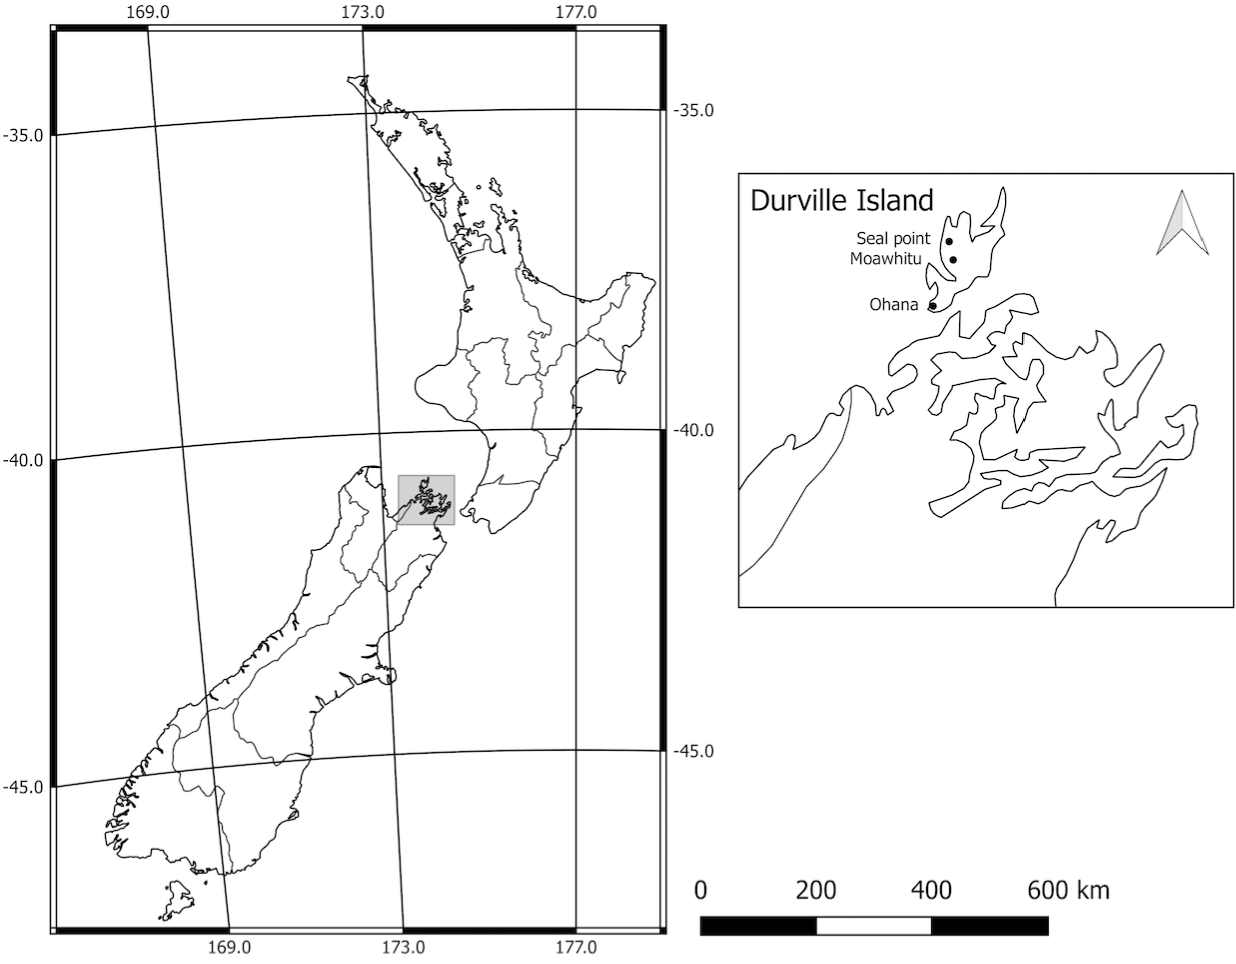
\includegraphics{figs/Durville.png}
\caption{Location of study sites (black circles), New Zealand{}}
\end{figure}

D'Urville's climate is maritime and consists of prevailing north-west
winds, reliable rainfall, frequent gales, mild winters and warm summers
(Walls 2009). Temperatures during the summer months of January to March
reach an average daily maximum of \(24^{\circ}\)C and are among the
warmest in the South Island of New Zealand. Typical winter daytime
temperatures are in the range \(10^{\circ}\)C - \(15^{\circ}\)C.
Drought-like conditions are sometimes experienced within the region. On
average, D'Urville Island receives over 1000mm of rain annually (NIWA
21AD--3AD).

The island's geology is comprised of igneous conglomerate, Permian
argillite and widespread areas of mafic and ultramafic rocks,
collectively known as the (Walls 2009) or the (Lee 1992). As a result,
the soils in parts of the island contain high concentrations of heavy
metals such as iron, copper, magnesium and nickel. Thus, it is a
component of the small (0.4\%) part of the NZ landmass that can be
described as (Lee 1992). The ultramafic areas create an environment
difficult for most plant species, and are characterised by unique plant
communities able to tolerate the high concentration of metallic minerals
in the soil.

D'Urville Island was an important cultural setting for early
Polynesians. Argillites strength and ability to hold a sharpened edge
made it ideal for making weapons and tools. Adzes, a tool dating back to
the Stone Age, commonly used to smooth or carve wood, were a key
instrument used for trade. Flakes of argillite dominate the occupation
layers in the cores analysed by (Wellman 1962), leading him to estimate
a total of 60 tonnes was extracted during the island's Polynesian
occupation, or enough to manufacture not less than 15,000 adzes,
acknowledging this is likely an underestimate due to the amount of
flakes still hidden. Lithic exchange was extremely important to
Polynesian settlers, and we see argillites from the northern South
Island appearing in the Bay of Plenty (central eastern New Zealand) less
than 10 years after quarries appearing on the landscape (Walter, Jacomb,
and Bowron-Muth 2010). The evidence suggests that D'Urville was the
centre of flourishing trade given the inferior quality of rock in other
parts of New Zealand. Midden deposits are found in every bay on
D'Urville Island, as are stone walls associated with gardens (Walls
2009). The occupation layer examined by (Wellman 1962) provides evidence
that horticulture was likely to have been prominent on the sandy flats,
as shown by the uniform distribution of pebbles associated with growing
kūmara (\emph{pomoea} spp).

The following vegetation descriptions have been summarised with
permission from (Walls 2009; Walls 2005); other descriptions also appear
in (Lee 1992) and (Beever, Brownsey, and Bellingham 1989). As with much
of New Zealand, human arrival on D'Urville Island brought about a
significant loss of native forest, and what remains can be best
described as a complex mosaic of exotic plantations, forest remnants,
pasture and areas undergoing secondary succession following clearing.
The most accessible and fertile low areas have, unsurprisingly, been
converted into grazed pasture, yet areas of fernland and shrub have
survived in the areas not suited to farming. The expansion of fern and
shrubland into previously grazed regions due to a cessation of farming
is noticeable in several areas and these are, predictably, dominated by
the early successional species such as \emph{Kunzea} spp.,
\emph{Leptospermum scoparium}, bracken (\emph{Pteridium esculentum}),
\emph{Cyathea medullaris}, \emph{Coprosma robusta}, \emph{Melicytus
ramiflorus} and \emph{Cordyline australis}. \emph{Fuscospora truncata}
dominates on many of the ridges and slopes from 500 m above sea level
(asl) to sea-level, often in association with \emph{Fuscospora
solandri}, \emph{Dacrydium cupressinum} and \emph{Elaeocarpus dentatus}.
At higher elevation, and in the cooler, moister areas, \emph{Fuscospora
truncata} is replaced by \emph{Lophozonia menziesii}, \emph{Lophozonia
fusca}, \emph{Prumnopitys ferruginea}, \emph{Metrosideros umbellata} and
other broadleaf species. Coastal flats and some coastal slopes, along
with gullies, contain many of the broadleaf species abundant throughout
of the North Island of New Zealand; of these species, \emph{Dysoxylum
spectabile} is most abundant, but \emph{Rhopalostylis sapida},
\emph{Laurelia novae-zelandiae}, \emph{Beilschmiedia tawa},
\emph{Alectryon excelsus}, \emph{Piper excelsum}, \emph{Aristotelia
serrata}, \emph{Hedycarya arborea}, \emph{Cyathea} spp. and
\emph{Carpodetus serratus} are common. Small examples of the low-forest
climax vegetation on ultramafic areas still exist, but are limited to
higher elevations and consist of \emph{Fuscospora truncata},
\emph{Dacrydium cupressinum}, \emph{Metrosideros umbellata},
\emph{Pseudopanax crassifolius} and \emph{Leptospermum scoparium}.
Although the ultramafic soils exclude many common woody weeds found in
the region, wilding pines such as \emph{Pinus contorta} and
\emph{Pseudotsuga menziesii} are invading some locations. D'Urville
Islands possum-free (\emph{Trichosurus vulpecula}) status has also
allowed for an abundance of mistletoe to adorn the island; also present
are examples of endangered species such as {Anemanthele lessoniana} and
\emph{Euphorbia glauca}. Mammalian pests associated with much of New
Zealand exist on D'Urville Island and include feral pigs (\emph{Sus
scrofa}), rodents, hedgehogs (\emph{Erinaceus europaeus occidentalis})
and mustelids (Walls 2009).

\section{Methods}\label{methods}

A D-section hand corer was used to collect a 250 cm long soil core from
Moawhitu Swamp. Cores from the lakes at Seal Point (143 cm length) and
Ohana (136 cm length) were collected using a simple gravity lake corer.

\subsection{Pollen Analysis}\label{pollen-analysis}

We subsampled 2 mL of soil from the Moawhitu Swamp core every 4 cm for
pollen analysis. Standard preparation techniques were used to make
microscope slides suitable for palynological analysis (Moore, Webb, and
Collison 1991). On each slide pollen from trees, shrubs, herbs and
bracken spores were recorded until a total of 250 grains was reached.
Reference collections (Landcare Research) and atlases (e.g. Moar 1993)
were used to identify pollen to the highest possible taxonomic
resolution. Distinct and unprecedented changes in vegetation and
charcoal inputs were used to isolate initial human activity. Pollen and
charcoal diagrams were constructed using the C2 software package
(Juggins 2007)

\subsection{Charcoal Analysis}\label{charcoal-analysis}

Charcoal was examined at high-resolution as per (Whitlock and Larsen
2002) to reconstruct local fire activity. Samples from Moawhitu Swamp,
Seal Point and Ohana cores were taken at contiguous 1 cm intervals using
a brass sampler with a rectangular cutting edge. Sub-samples were taken
at a volume of 2 cm\(^{3}\) where sufficient material was available, and
1 cm\(^{3}\) if not in the Moawhitu Swamp core. At both Seal Point and
Ohana sub-samples were taken at a volume of 5 cm\(^{3}\). All samples
were soaked in 6\% bleach for 24 hours. At Moawhitu Swamp samples were
washed through Petri dishes 250 , 125 and 63 , at Seal Point and Ohana
samples were washed through 125 Petri dishes. Charcoal particles were
counted using a stereomicroscope at 50-100x magnification. Charcoal
concentration (number of particles/cm\(^{3}\)) was determined using
total charcoal counts divided by the volume of sediment sieved. Charcoal
accumulation rates were calculated by dividing charcoal concentration by
deposition time (yr/cm) between each sample.

\subsection{Radiocarbon dating}\label{radiocarbon-dating}

We submitted three twig samples from the Moawhitu Swamp core to the
Waiakto Radiocarbon Dating Laboratory, New Zealand for accelerator mass
spectrometry (AMS) radiocarbon dating. Ages of all dated material are
expressed as calibrated \(^{14}\)C age before present (cal. year BP).
The samples from Moawhitu Swamp were taken from 32 cm, 59 cm and 94 cm.
Three cal. year BP dates were supplied from Ohana at 94 cm, 103 cm and
122 cm, and three from Seal Point at 80 cm, 105 cm and 115 cm. These
dates are courtesy of Dr. David McWethy, Montanta State University, USA.
Age-depth modelling, as per the algorithm of (Haslett and Parnell 2008)
and the Southern Hemisphere (SHCal13) calibration curve (Hogg et al.
2013), were constructed using the Bchron package (Parnell 2014) in the R
statistical suite (R Core Team 2015) version 3.1.3 (Fig:
{[}fig:age-depth-model{]}).

\begin{figure}
\centering
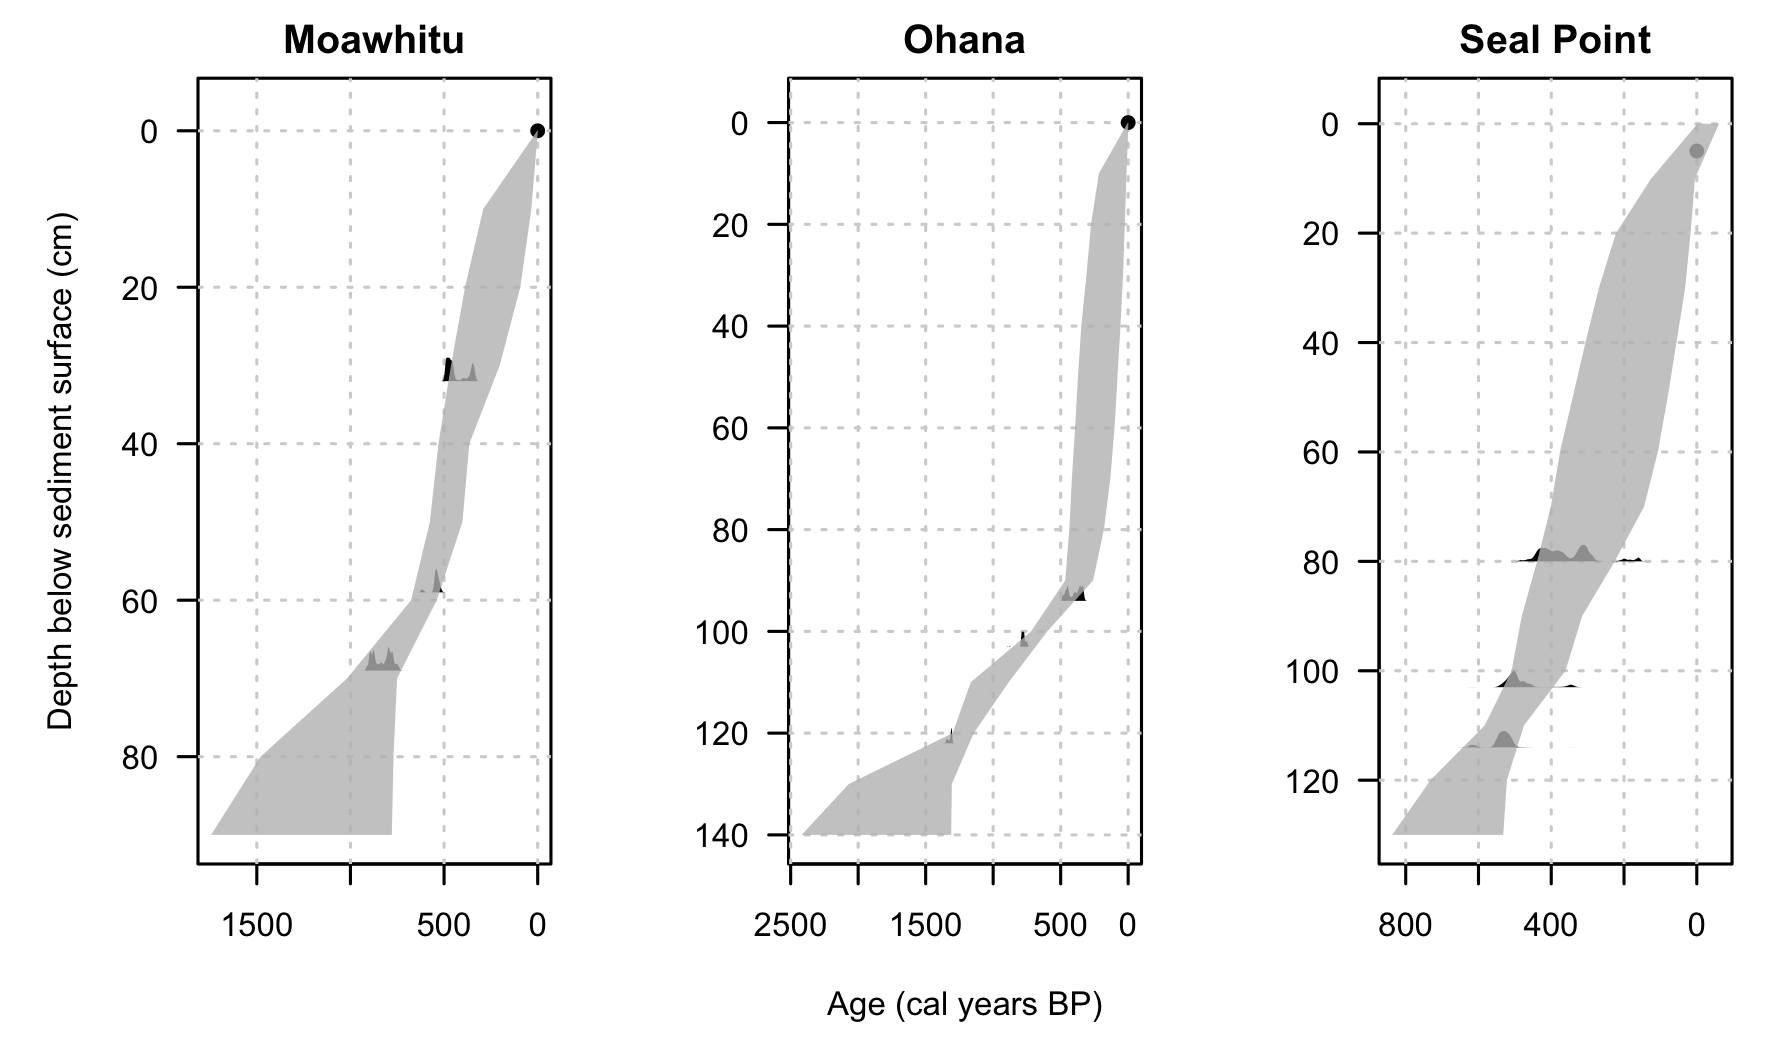
\includegraphics{Figs/age-depth-models/age-depth-model-all.png}
\caption{Age depth models for each site constructed using the compound
Poisson-Gamma chronology model of (Haslett and Parnell 2008). Light grey
distributions indicate probability distributions from calibrated
\(^{14}\)C dates.{}}
\end{figure}

\subsection{Statistical analysis}\label{statistical-analysis}

Statistical analysis was conducted using the R statistical package (R
Core Team 2015), version 3.2.3. Constrained cluster analysis that
honoured the location of sites (CONISS), and nMDS ordination, using the
Bray-Curtis measure (Faith, Minchin, and Belbin 1987) were performed on
the pollen reconstruction from Moawhitu Swamp using the rioja (Juggins
2015) and VEGAN (Dixon and Palmer 2003) packages. Permutational
multivariate analysis of variance (PERMANOVA) using distance matrices
(Anderson 2001) were performed using the adonis command to statistically
evaluate the dissimilarity between settlement and prehuman zones.
Temporal auto-correlation between charcoal and magnetic susceptibility
was conducted using the acf and ccf functions.

\subsection{Magnetic Susceptibility}\label{magnetic-susceptibility}

Not sure of the methods here.... Only for Seal Point and Ohana

\section{Results}\label{results}

The timing of human arrival was estimated using a combination of
distinct changes in pollen taxa (e.g. the introduction of exotic
species), charcoal reconstructions and accompanied by statistical
analysis of the pollen reconstruction from Moawhitu Swamp. Three zones
were initially identified as a result of nMDS ordination on pollen taxa
from the Moawhitu Swamp core: Zone 3 (0-20 cm, 0-125 cal. years BP),
zone 2 (20-64 cm, 150-650 cal. years BP) and zone 1 (64-250 cm, 650-2200
cal. years BP) (Fig: {[}fig:ordination{]}). Vegetation changes are
demonstrated by a rapid rise in bracken and Poaceae, accompanied by a
decrease in native forest taxa (Fig: {[}fig:podo-beach-tree{]},
{[}fig:ferns{]}, {[}fig:disturbance{]}), and the increase of charcoal
into the Moawhitu Swamp, Seal Point and Ohana cores (Fig:
{[}fig:podo-beach-tree{]}, {[}fig:charcoal-ohana{]},
{[}fig:charcoal-seal{]}).

\begin{figure}
\centering
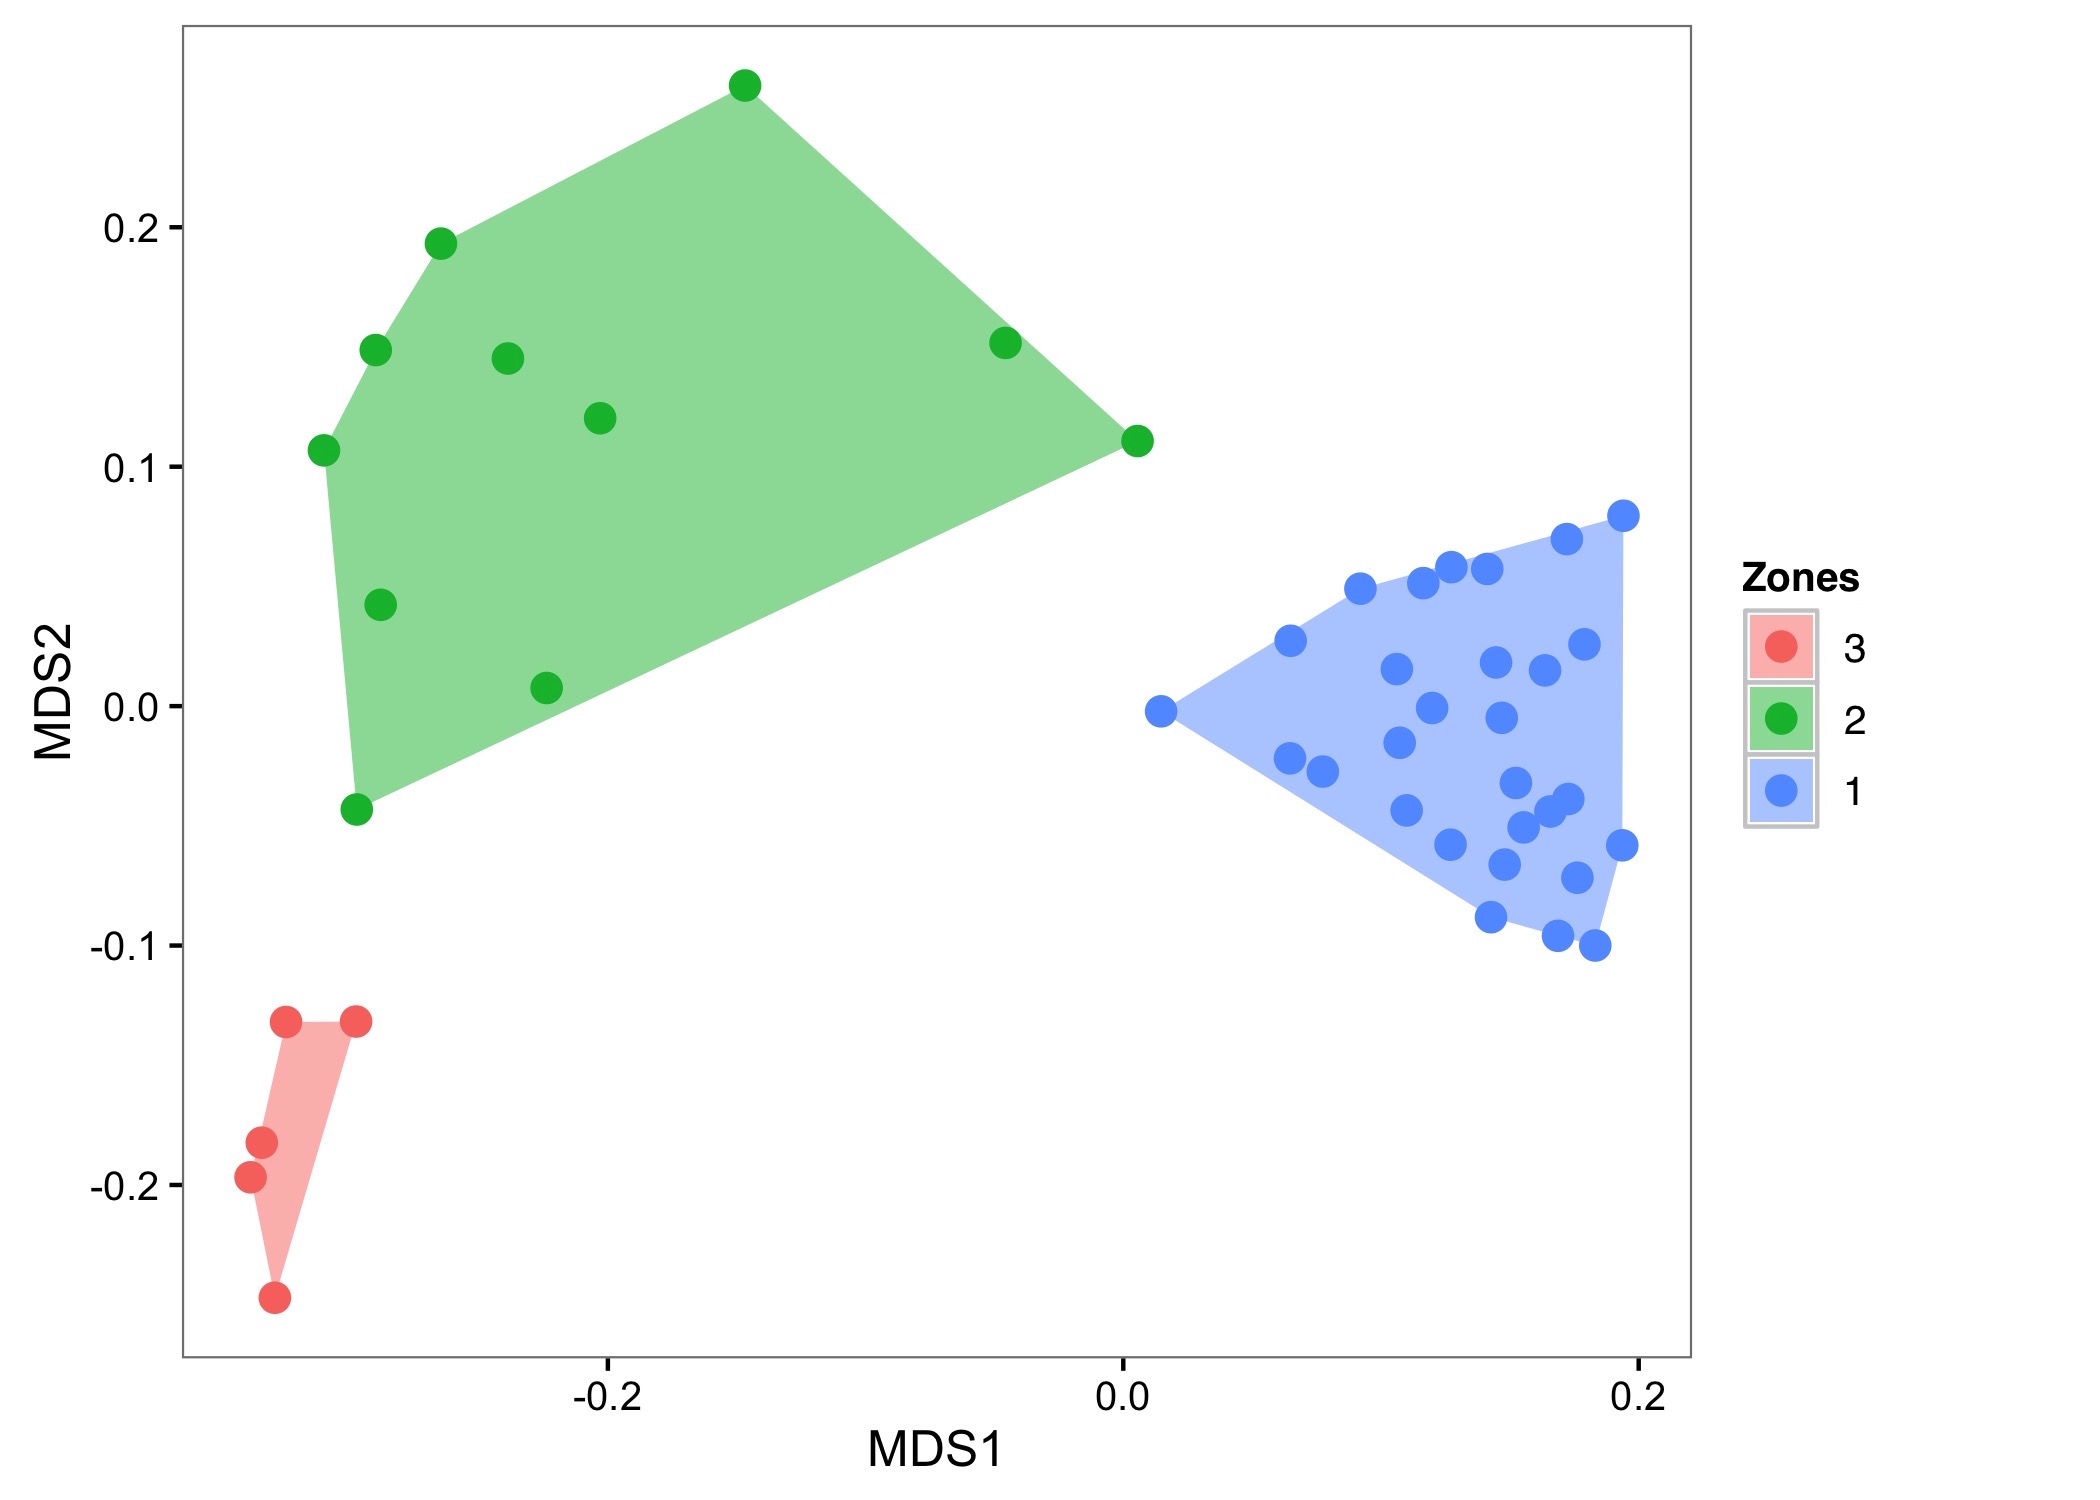
\includegraphics{Figs/nmds-analysis.jpeg}
\caption{nMDS Ordination of settlement and prehuman zones identified
from cluster analysis. Zones identified by different colors. Stress
level = 0.1. Polygons indicate minimum bounding box.{}}
\end{figure}

\subsection{Zone 1 - 650 - 2120 cal. years
BP}\label{zone-1---650---2120-cal.-years-bp}

Based on the pollen present, zone 1 comprises a
Nothofagaceae-\emph{Podocarpus} mosaic with a broadleaf sub-canopy and a
ground layer of ferns (Fig: {[}fig:podo-beach-tree{]}, {[}fig:ferns{]}).
Also notable is the presence of \emph{Rhopalostylis sapida} and
\emph{Dysoxylum spectabile}, which is indicative of a rich coastal, lake
and wetland forest. There are no discernible shifts in vegetation during
this part of the core and pollen sum percentages remain relatively
consistent. The podocarp taxa are the most variable component of the
palynoflora (Fig: {[}fig:podo-beach-tree{]}).

\begin{figure}
\centering
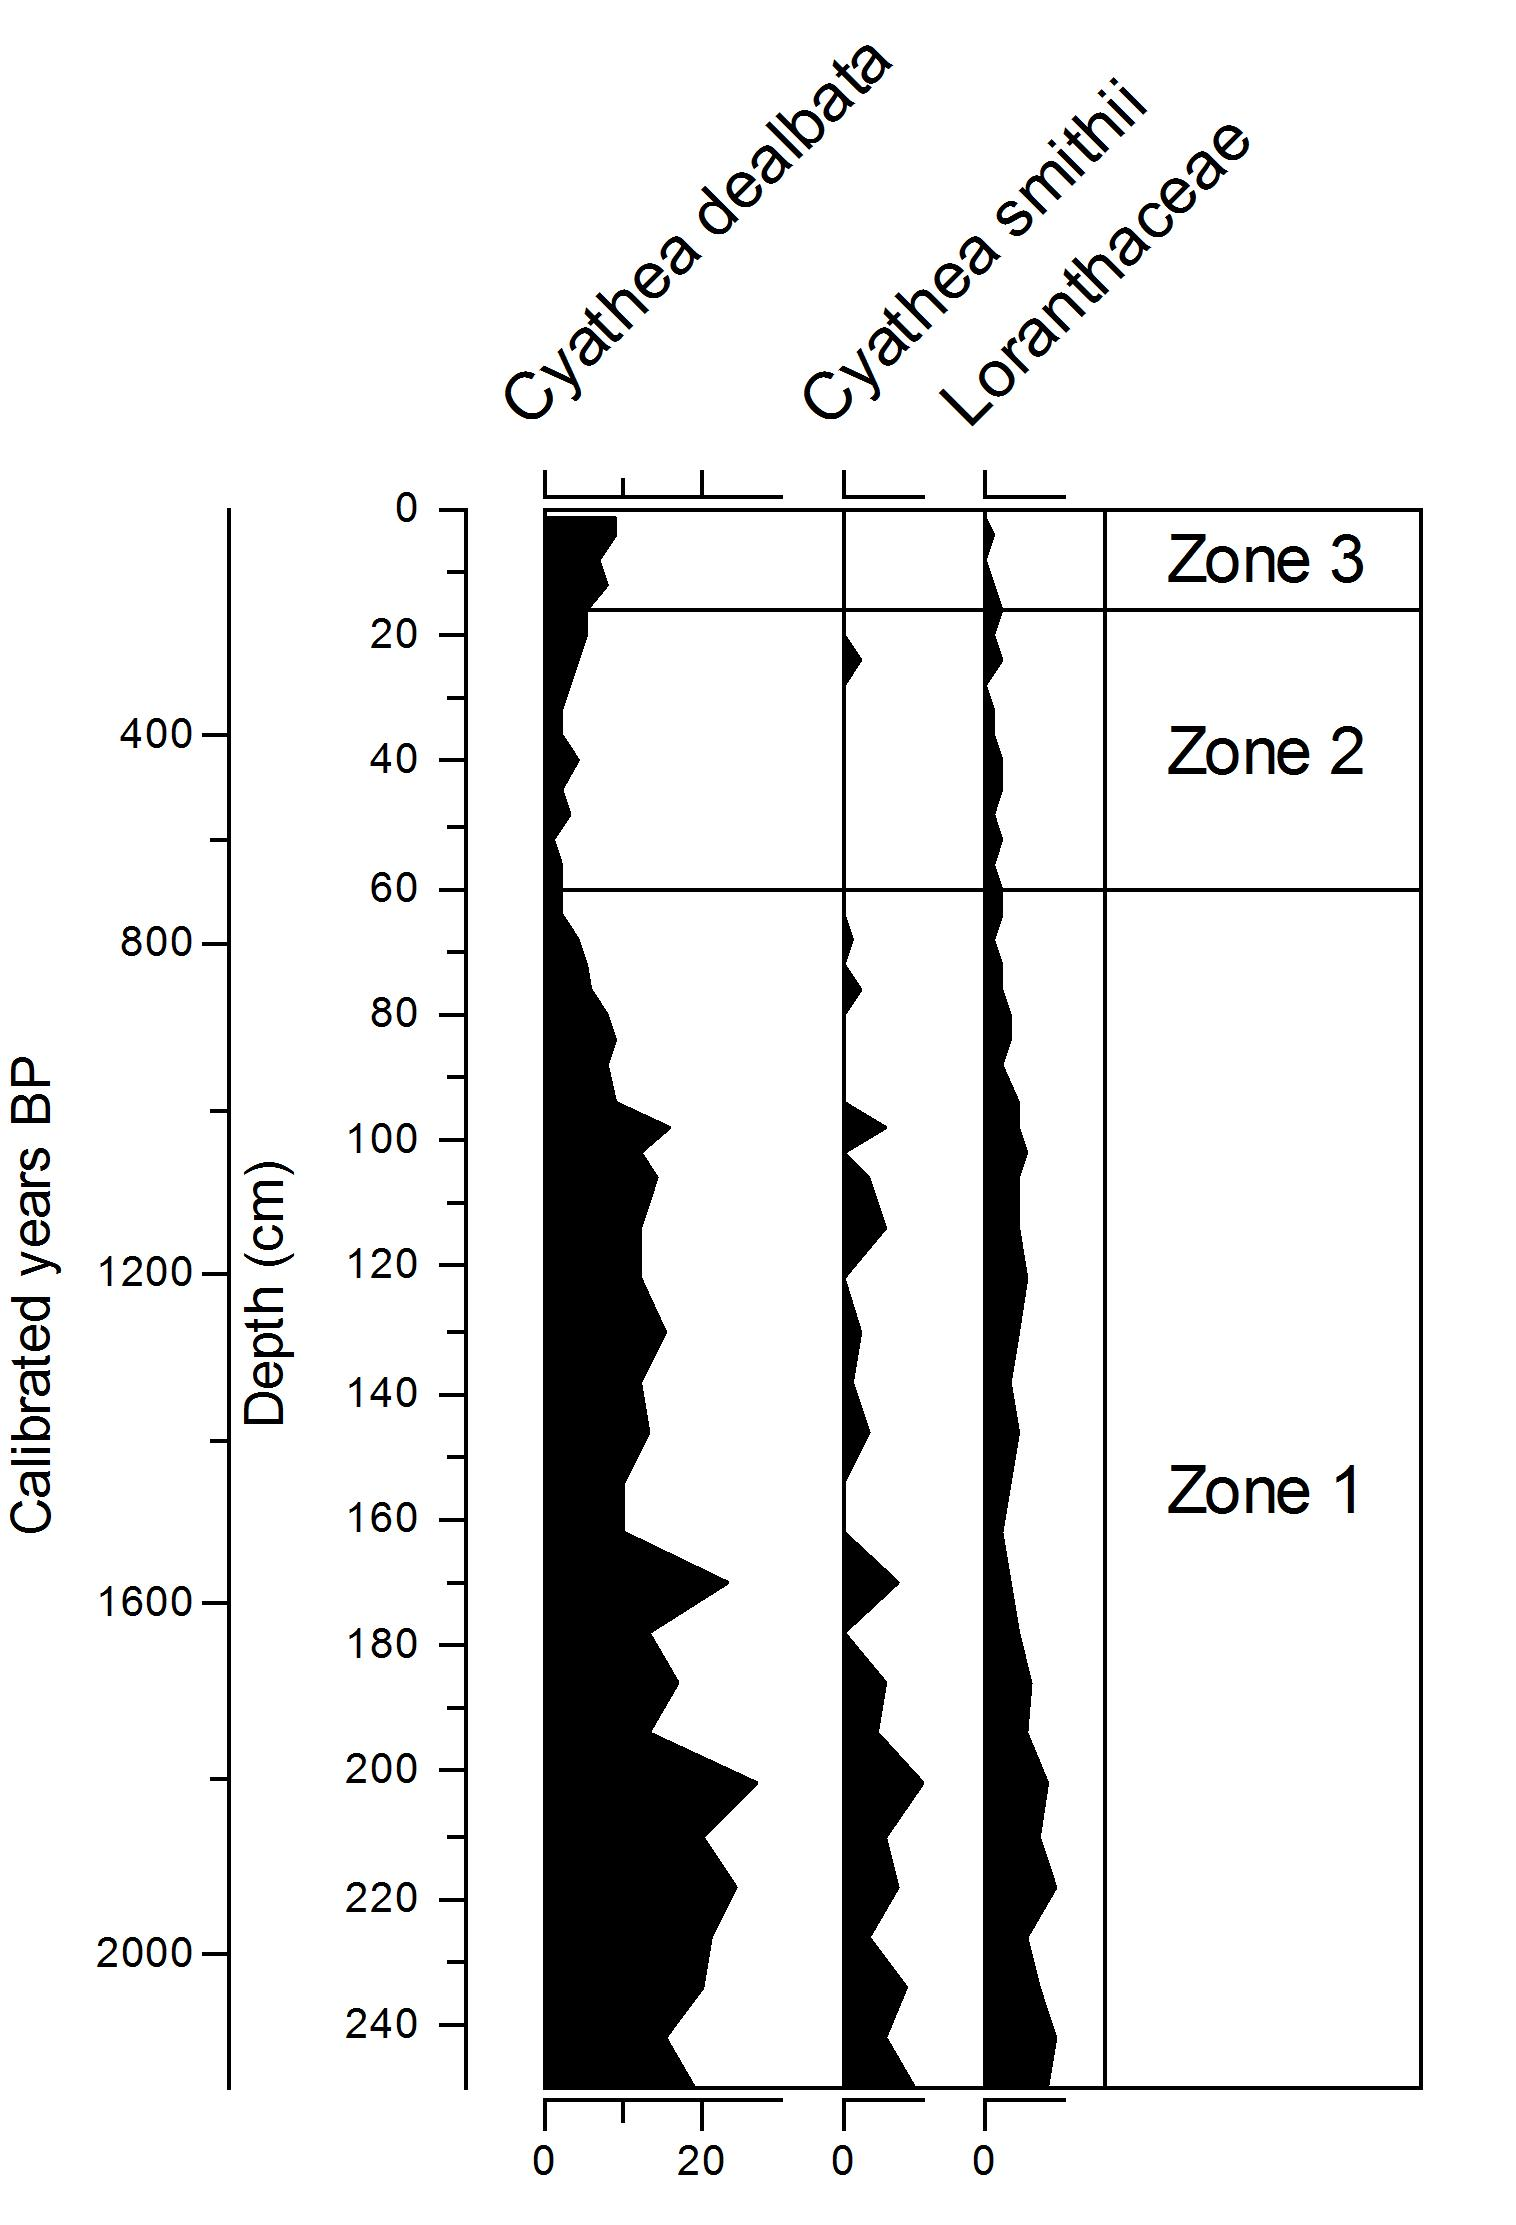
\includegraphics{ferns-zone.jpg}
\caption{Ferns and mistletoe identified in the pollen reconstruction
from Moawhitu Swamp. Pollen sum given as a percentage of total pollen
count.{}}
\end{figure}

\subsection{Zone 2 - 150 - 650 cal. years
BP}\label{zone-2---150---650-cal.-years-bp}

The decline in podocarps as forest was cleared is an indication of
change in zone 2 from zone 1 (Fig: {[}fig:podo-beach-tree{]},
{[}fig:disturbance{]}). The biggest drivers of this difference are the
decrease in podocarps, and increase in grasses and bracken, as forest
taxa are replaced by disturbance-tolerant species. The creation of young
and seral forest is evident in the increase in \emph{Leptospermum
scoparium} and \emph{Cordyline} pollen (Fig: {[}fig:podo-beach-tree{]},
{[}fig:disturbance{]}). Large fire events during this period are
evidenced by spikes in bracken, \emph{Typha} and monolete fern spores.

\begin{figure}
\centering
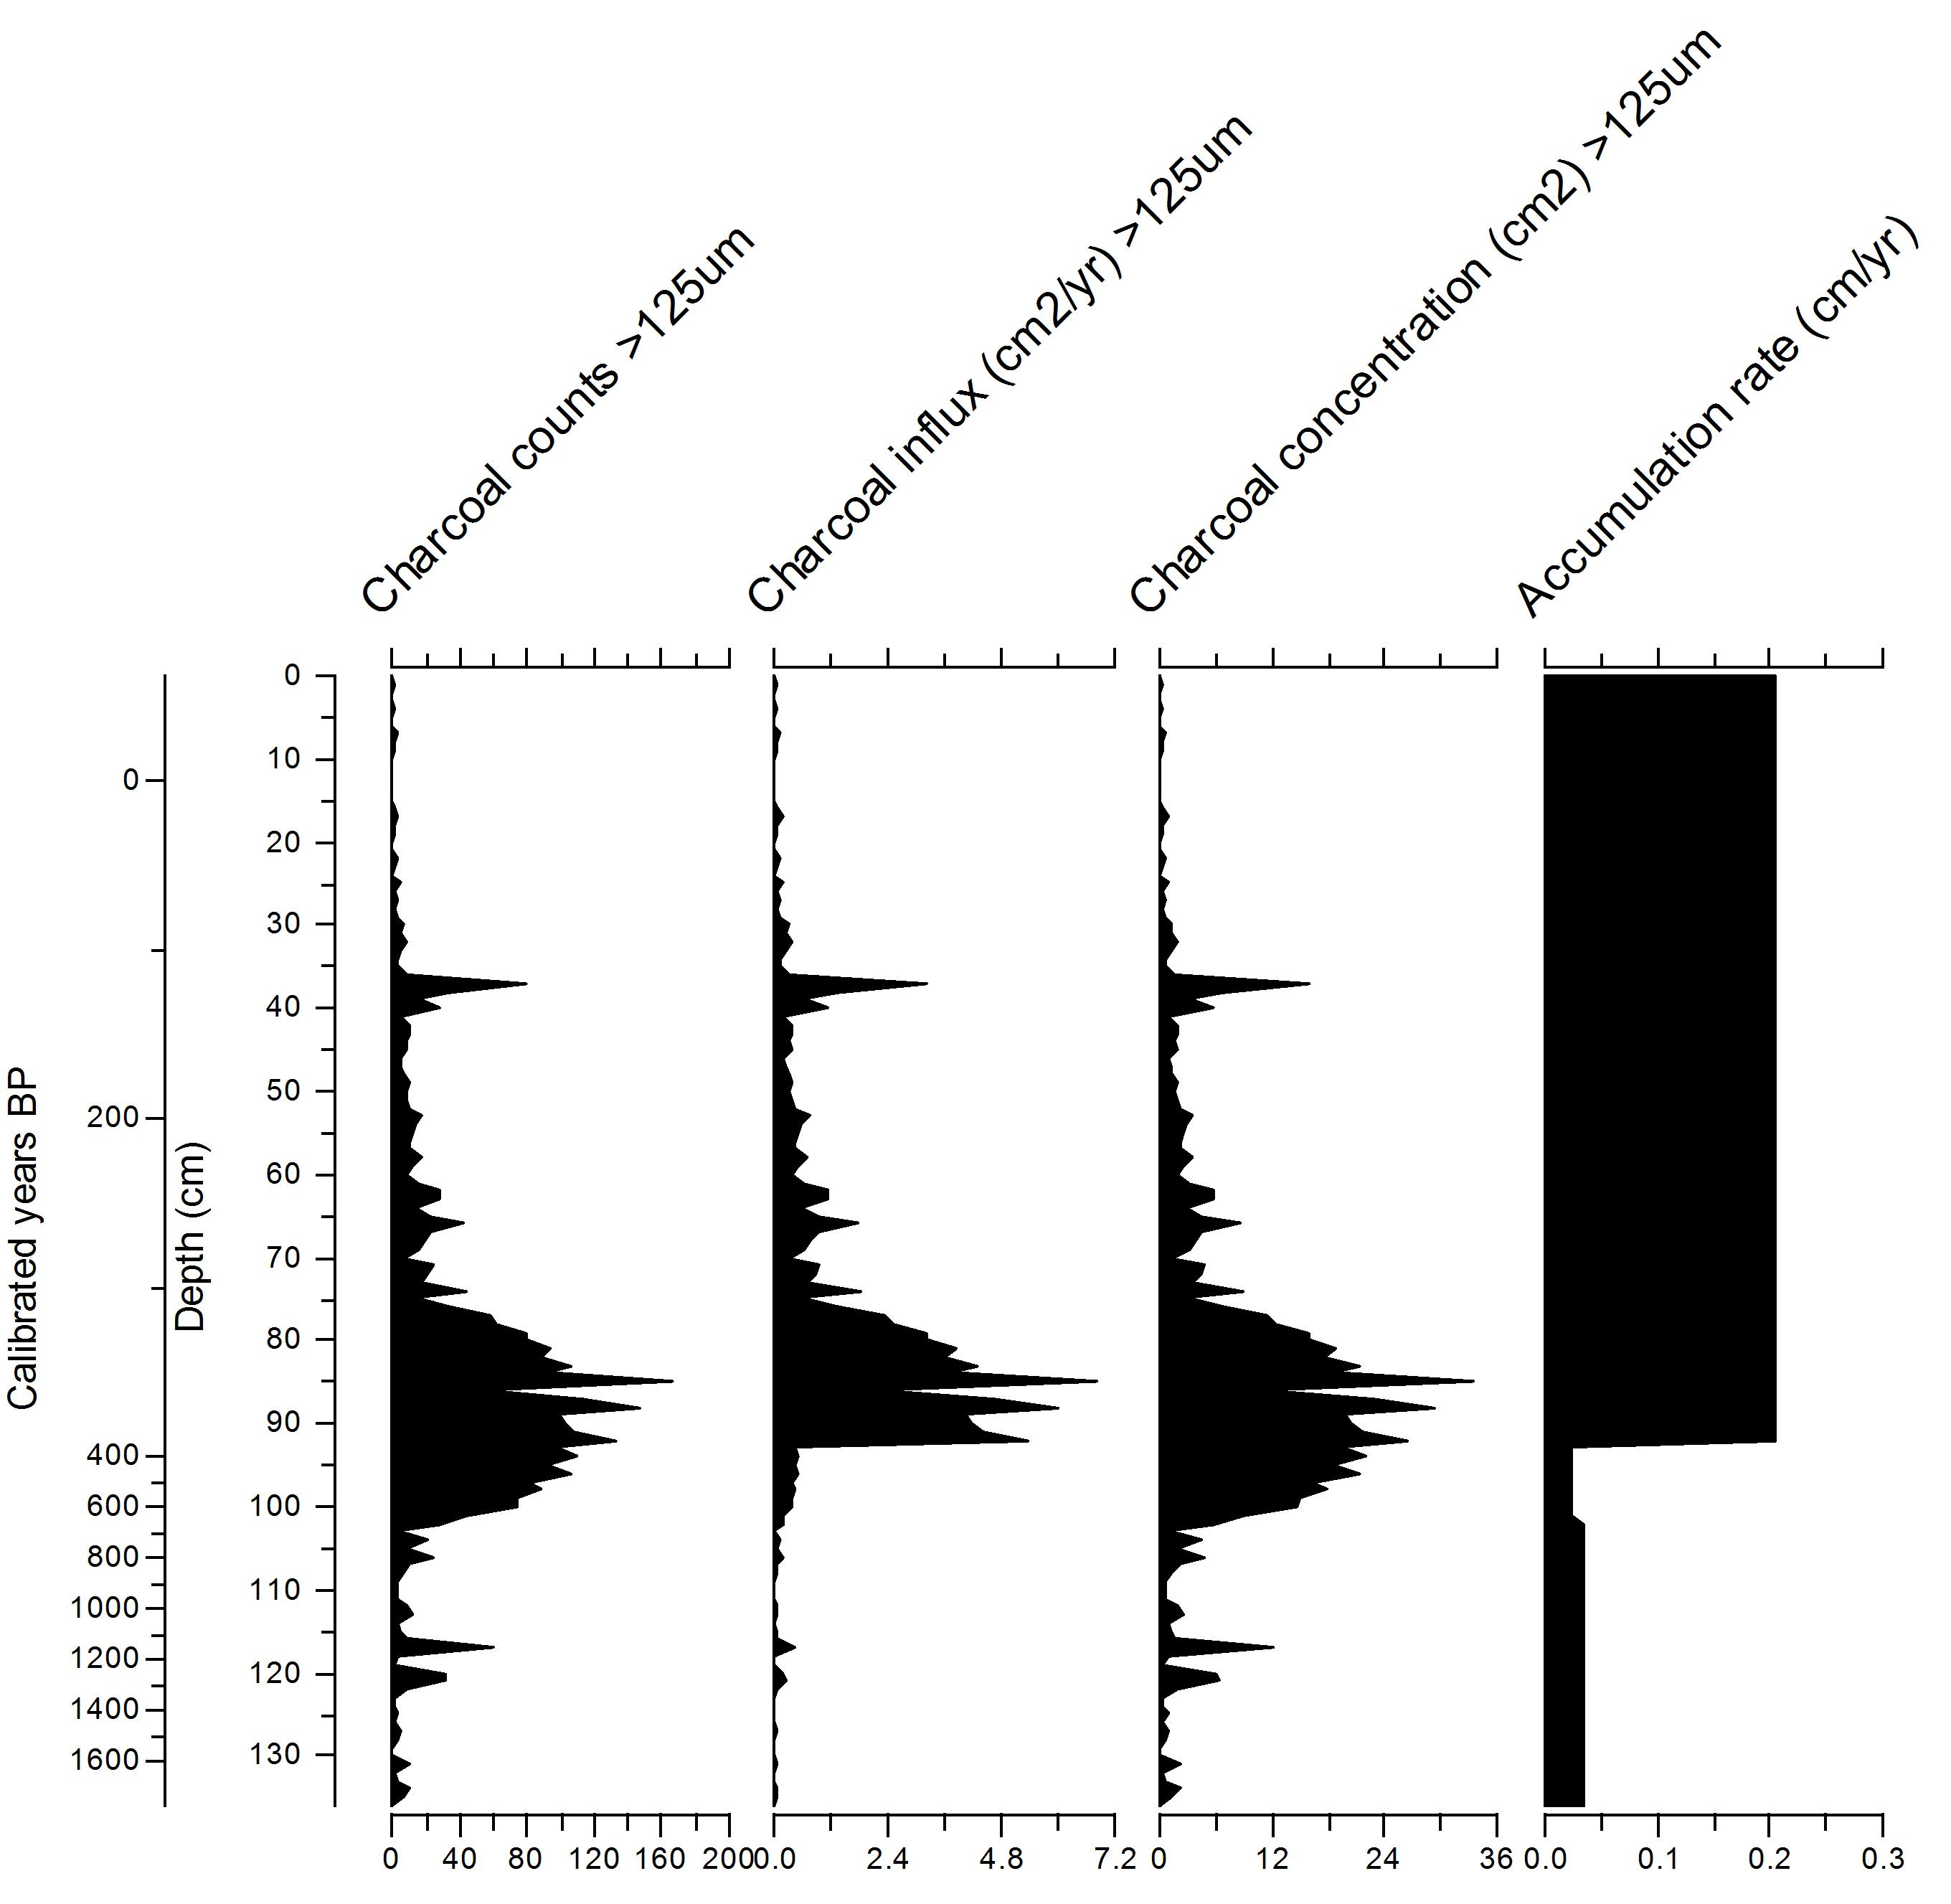
\includegraphics{ohana.jpg}
\caption{Macroscopic charcoal from the Ohana profile, expressed as
concentrations and influx. Sedimentation rates expressed as accumulation
(cm/yr).{}}
\end{figure}

\begin{figure}
\centering
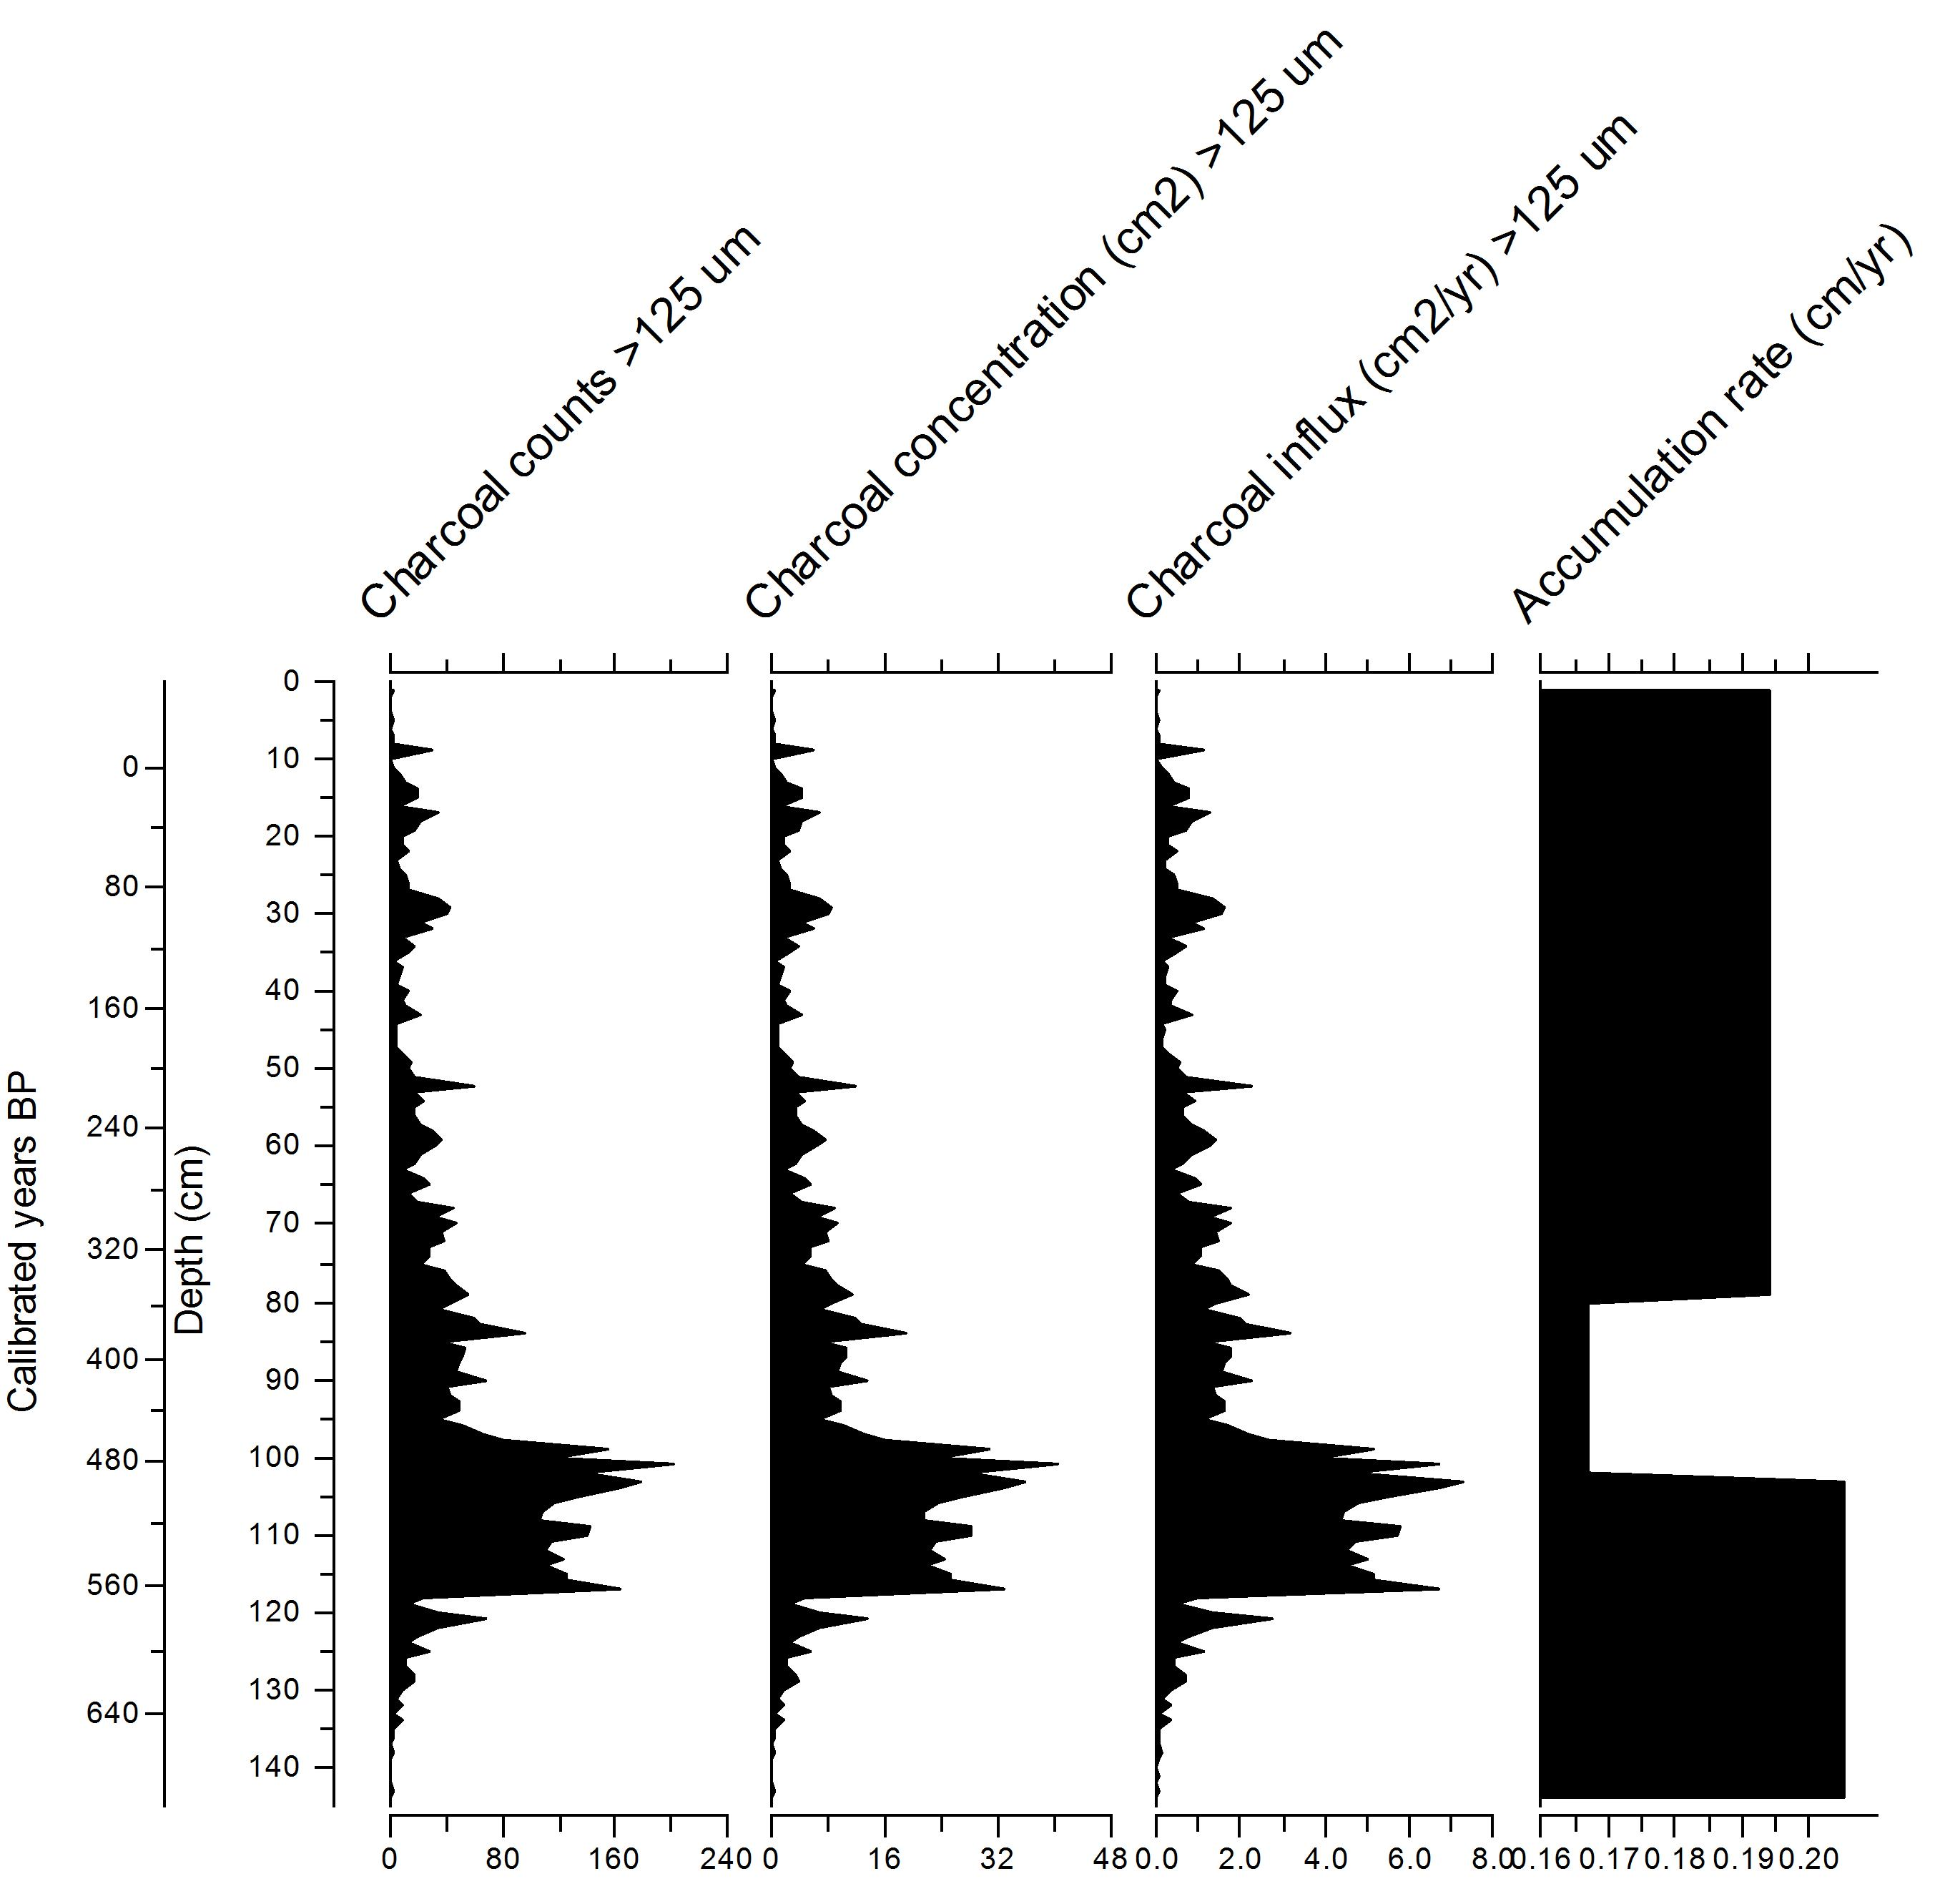
\includegraphics{seal.jpg}
\caption{Macroscopic charcoal from the Seal Point profile, expressed as
concentrations and influx. Sedimentation rates expressed as accumulation
(cm/yr).{}}
\end{figure}

\subsection{Zone 3 - 0 -150 cal. years
BP}\label{zone-3---0--150-cal.-years-bp}

The arrival or establishment of several exotic species, including
\emph{Taraxacum} spp., \emph{Pinus} spp., and the non-native
\emph{Plantago}, marks zone 3. Pollen of disturbance-related taxa such
as bracken, \emph{Typha} spp., and monolete fern spores contribute most
to the differences observed. Monolete fern spores and \emph{Typha}
decline during this modern period and this is likely due to the
reduction in fire-related disturbance events (Fig:
{[}fig:podo-beach-tree{]}, {[}fig:disturbance{]}). Exotics, such as
\emph{Pinus} and non-native \emph{Plantago}, are also important
contributors to the different vegetation communities observed. Forest
taxa, particularly podocarps, have the lowest pollen sum percentage
observed across all three zones. The open forest favours the growth of
light-demanding and pioneer species such as \emph{Leptospermum
scoparium}, \emph{Kunzea} spp. and \emph{Cordyline}.

\subsection{Sediment-charcoal records}\label{sediment-charcoal-records}

Charcoal is absent from much of zone 1 in the Moawhitu Swamp core (Fig:
{[}fig:podo-beach-tree{]}). Consistent inputs of microscopic charcoal at
Moawhitu Swamp begin around 1100 cal. years BP, with three peaks at c.
490, 470 and 228 cal. years BP. All three sites show increasing
macroscopic charcoal inputs from around 650 cal. years BP onwards, with
charcoal concentrations being highest from 400 - 600 cal. years BP (Fig:
{[}fig:podo-beach-tree{]}, {[}fig:charcoal-ohana{]},
{[}fig:charcoal-seal{]}). The Ohana Lake profile also exhibits another
charcoal peak at 120 cal. years BP after a steady decline, with Seal
Point also showing higher concentrations around this period (Fig:
{[}fig:charcoal-ohana{]}, {[}fig:charcoal-seal{]}). The Moawhitu Swamp
core is more temporally variable in terms of charcoal concentration, but
shows a similar pattern of increased burning at around 100 cal. years BP
(Fig: {[}fig:podo-beach-tree{]}). A visual comparison of charcoal
concentration and influx from the Moawhitu and Seal Point cores reveals
close agreement in temporal pattern across size classes (Fig:
{[}fig:podo-beach-tree{]}, {[}fig:charcoal-seal{]}). A dramatic increase
in accumulation after nearly three centuries of increased charcoal
inputs correlates with increases in charcoal influx just after 400 cal.
years BP in the Ohana core (Fig: {[}fig:charcoal-ohana{]}).

\subsection{Magnetic susceptibility}\label{magnetic-susceptibility-1}

Corresponding with Polynesian arrival, magnetic susceptibility increases
from c. 600 cal. years BP in the Seal Point core. This rise in magnetic
susceptibility peaks c. 175 years later, and then shows a fluctuating
decline until European arrival (c. 150 cal. year BP), when magnetic
susceptibility increases until a peak c. 120 cal. years BP, gradually
declining thereafter. Polynesian settlement does not give a clear signal
in the Ohana core, with magnetic susceptibility declining c. 600 cal.
years BP. This decline continues for c. 200 years before we see
increases to the highest magnetic susceptibility levels seen in the
core. European settlement provides a clearer signal in the Ohana core,
with similar magnetic susceptibility increases c. 150 cal. years BP to
those in Seal Point. Charcoal and magnetic susceptibility were not
significantly correlated in either the Seal Point or Ohana profiles,
(r=0.179 and r=0.157, respectively), however there is a significant
lagged correlation between fire activity (as measured by charcoal) and
magnetic susceptibility. The maximum correlation occurs when a lag of 22
cm is applied (r=0.541, P \textless{}0.05) or approximately 60 years to
the Seal Point core. Correlation also improves (r=0.547, P
\textless{}0.05) when a 50 year lag is applied to the Ohana profile.

\begin{figure}
\centering
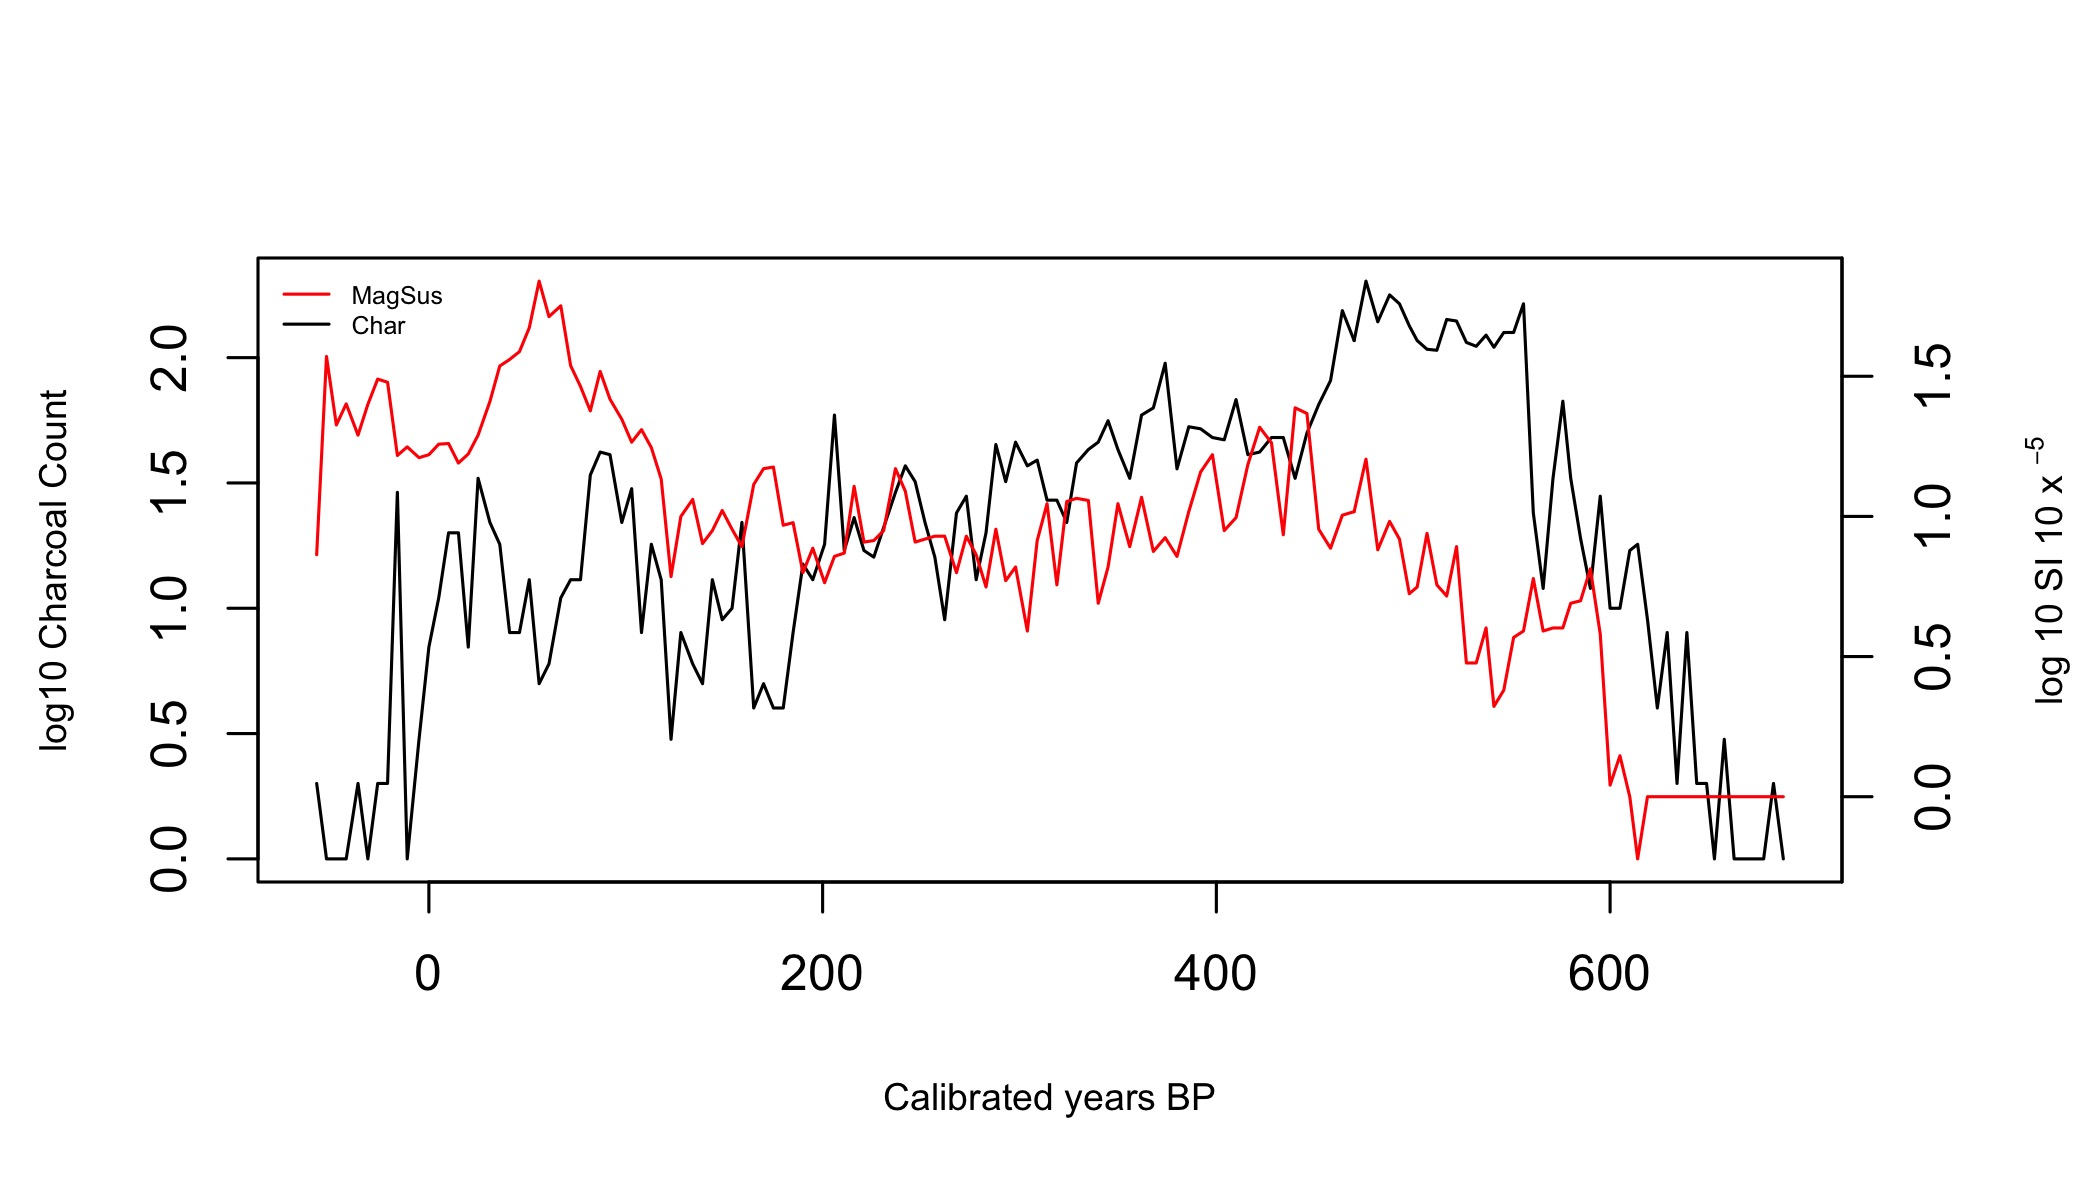
\includegraphics{mag-sus-seal.jpeg}
\caption{Magnetic susceptibility (log10) and charcoal particle count
(log10) from the Seal Point core.{}}
\end{figure}

\begin{figure}
\centering
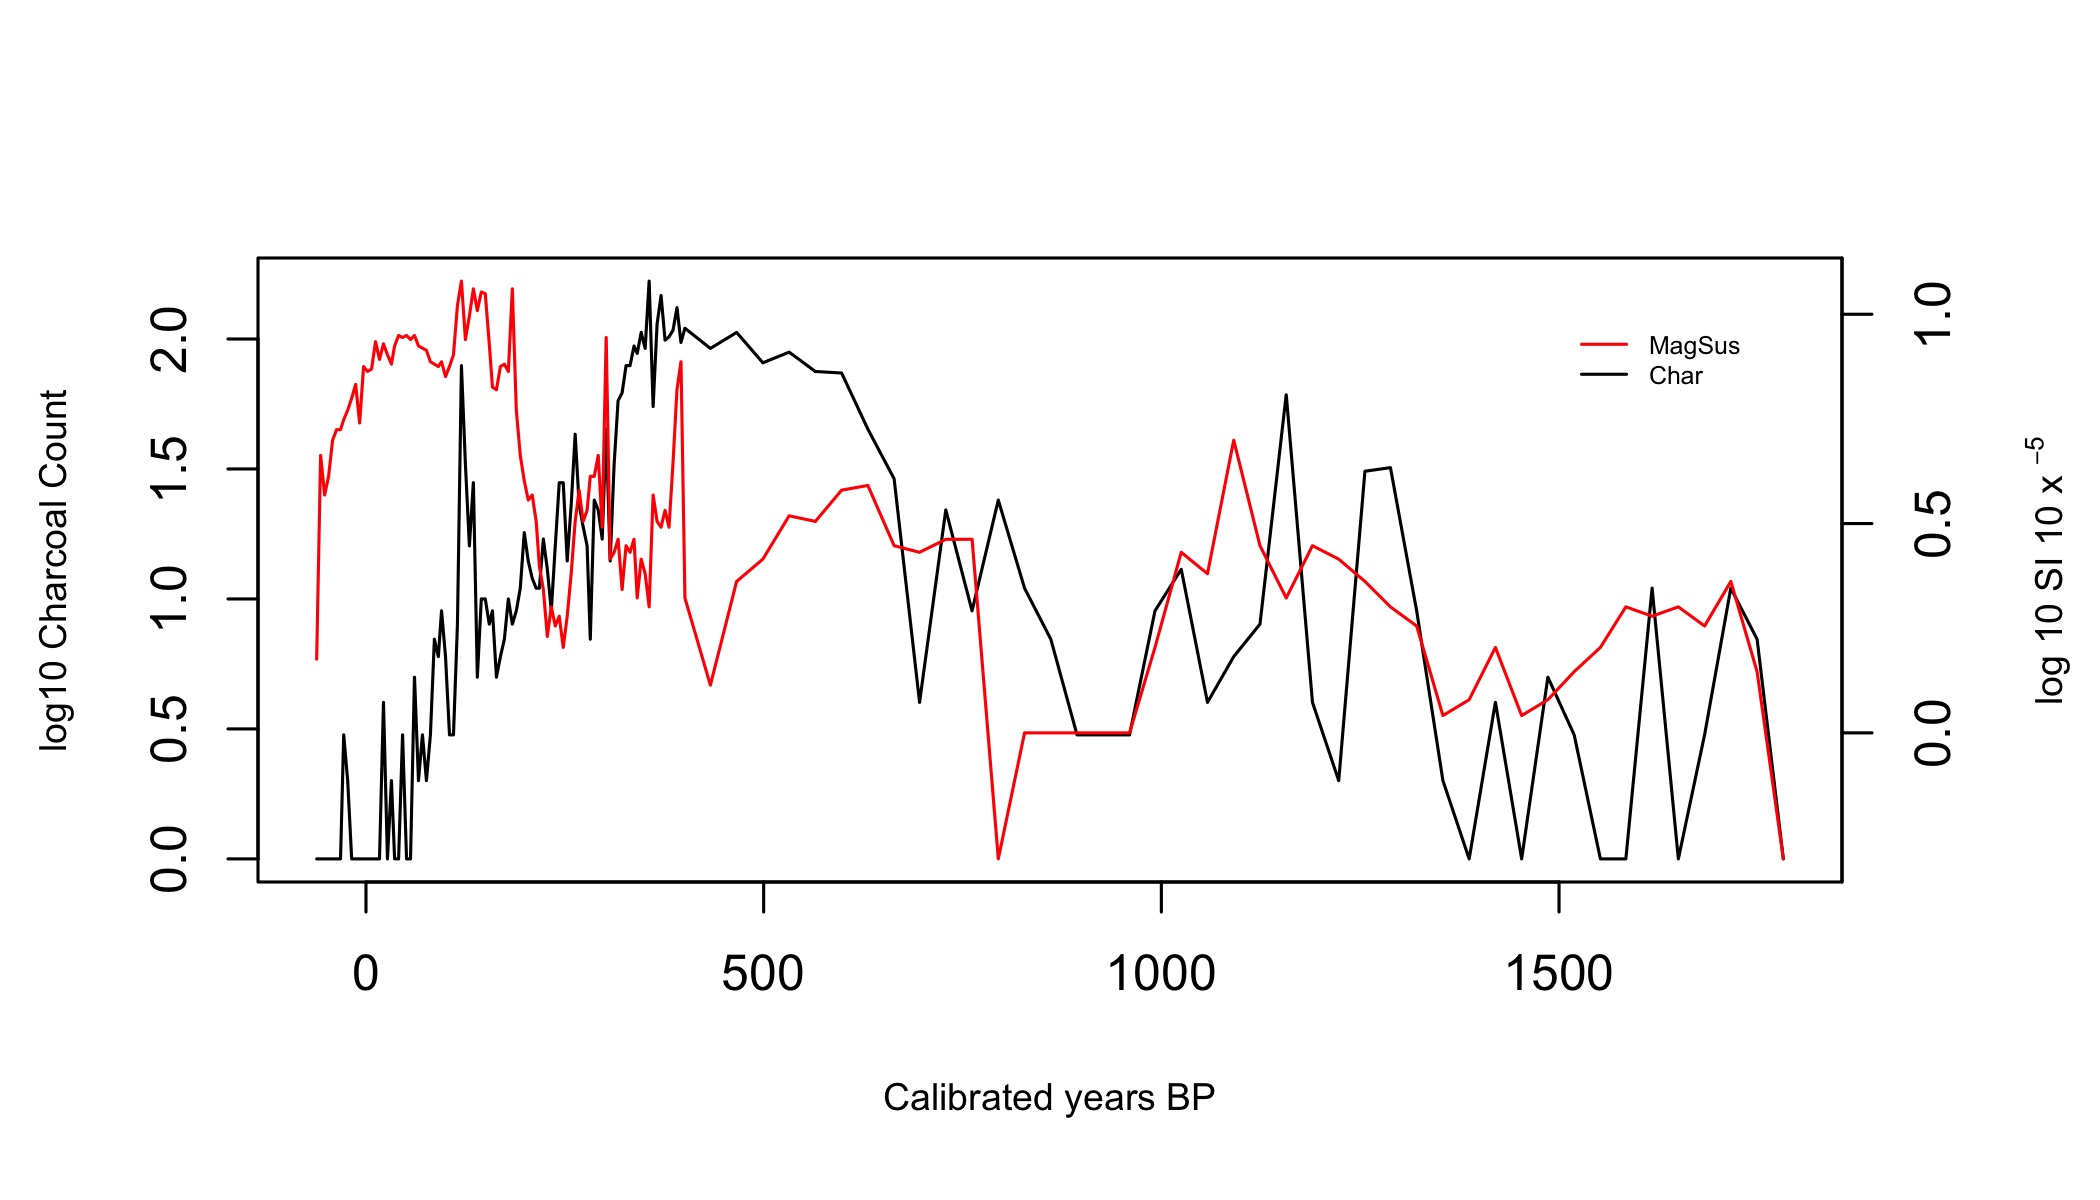
\includegraphics{mag-sus-ohana.jpeg}
\caption{Magnetic susceptibility (log10) and charcoal particle count
(log10) from the Ohana core.{}}
\end{figure}

\subsection{Definition of settlement and prehuman zones using all
proxies}\label{definition-of-settlement-and-prehuman-zones-using-all-proxies}

Previous work by (Wilmshurst et al. 2008) places Polynesian settlement
of New Zealand at c. 1280 AD. Based on the combination of sustained
burning, decline of forest (Fig: {[}fig:podo-beach-tree{]}) and increase
in disturbance related taxa in the pollen record (Fig:
{[}fig:disturbance{]}), settlement of D'Urville Island likely began c.
650 cal years BP, corresponding to a depth of c. 64 cm in the Moawhitu
Swamp core (Fig: {[}fig:disturbance{]}). This Polynesian settlement
period represents zone 2 in the ordination presented
(Fig:{[}fig:ordination{]}), and shall be referred to as such hereafter;
zone 1 will be identified as prehuman (Table: {[}t:zone-name{]}).

Exotic pollen taxa are a clear signal of European settlement and so
their arrival c. 150 cal. years BP make the European zone easier to
identify. \emph{Pinus}, non-native \emph{Plantago} and \emph{Taraxacum}
appear at 20 cm in the Moawhitu Swamp core. Unfortunately, the lack of
radiocarbon dates towards the top of all three cores, combined with the
notorious difficulty in dating periods ranging from 1800 to 1950 AD
(Hajdas 2008) (a result of increases in fossil fuel combustion during
the industrial revolution), creates a high degree of uncertainty in this
zone. However, reliable records show permanent European settlement of
D'Urville Island followed that of other New Zealand locations in 1840
AD, with the arrival of the first immigration ships at Port Hardy (a
large inlet to the north of D'Urville Island) (Walls 2009). Given these
historical dates for European arrival, and the appearance of exotic taxa
in the pollen reconstruction, it is safe to assume that European arrival
occurred at around 20 cm (c. 150 cal. years BP), encompassing zone 3
(Fig: {[}fig:ordination{]}). The relevant depths, mean cal. years BP,
zone numbers and subsequent names are given in Table {[}t:zone-name{]}.

{[}t:zone-name{]}

\begin{longtable}[]{@{}cccc@{}}
\caption{Zones identified as a result of age-depth model, pollen and
charcoal analysis from all three cores.}\tabularnewline
\toprule
Depth (cm) & Mean estimate of cal. years BP & Zone Number & Zone
Name\tabularnewline
\midrule
\endfirsthead
\toprule
Depth (cm) & Mean estimate of cal. years BP & Zone Number & Zone
Name\tabularnewline
\midrule
\endhead
0 - 20 cm & 0 - 150 & 3 & European\tabularnewline
20 - 64 cm & 150 - 650 & 2 & Polynesian\tabularnewline
64 - 250 cm & 650 - 2120 & 1 & Prehuman\tabularnewline
& & &\tabularnewline
\bottomrule
\end{longtable}

\section{Discussion}\label{discussion}

Analysis of the data from the three sites considered in this study
provide a first look at the late Holocence vegetation and fire history
of D'Urville Island in the Marlborough Sounds, New Zealand. Pollen
assemblages, macroscopic and microscopic charcoal in the sediment
profile from Moawhitu Swamp provide a 2200 year record of vegetation
shifts and fire history. Cores taken from Seal Point and Ohana Lake date
back to c. 688 and c. 1782 cal. years BP, respectively. This study
confirms that fire was a rare event prior to human arrival on the
island, but c. 650 cal. year BP, and coincident with human arrival, it
dramatically increased. The introduction of exotic plant species
following European arrival c. 150 cal. year BP further complicates an
already highly altered ecosystem.

\subsection{What were the pre-human plant
assemblages?}\label{what-were-the-pre-human-plant-assemblages}

The lack of change in pollen percentages during the pre-human zone
suggests relatively stable vegetation assemblages (Fig:
{[}fig:podo-beach-tree{]}). It is unlikely that large disturbance events
on D'Urville Island occurred with any frequency prior to human
settlement, although it has been suggested that a tsunami struck the
island around the 16\textsuperscript{th} century (Mitchell and Mitchell
2007); however, there is no evidence in the pollen reconstruction for
such an event. We see a clear and persistent dominance of Nothofagaceae
throughout the pre-human period, on average accounting for over 50\% of
the total pollen sum (Fig: {[}fig:podo-beach-tree{]}). During this
pre-human period Nothofagaceae forest is associated with a tall emergent
layer of podocarp species including \emph{Dacrydium cupressinum},
\emph{Dacrycarpus dacrydioides}, \emph{Prumnopitys ferruginea},
\emph{Prumnopitys taxifolia} and \emph{Podocarpus totara}. This
Nothofagaceae-\emph{Podocarpus} forest would have been accompanied by a
diverse canopy of \emph{Weinmannia} spp., \emph{Nestegis} spp. and
\emph{Elaeocarpus} spp. Smaller trees in the sub-canopy include
\emph{Coprosma} spp., \emph{Alectryon excelsus} and \emph{Dodonaea
viscosa}. Climbers such as \emph{Rubus} spp. also occur in the pollen
record. Shrubs associated with forest margins including
\emph{Aristotelia} spp., \emph{Melicytus} spp., \emph{Pseudopanax} spp.,
\emph{Myrsine} spp., \emph{Coprosma} spp., \emph{Rubus} spp., and
bracken are consistent throughout. \emph{Dysoxylum spectabile},
\emph{Aristotelia serrata}, \emph{Rhopalostylis sapida} and
\emph{Leptospermum scoparium} would have been abundant, likely on
coastal slopes and gullies. Tree-ferns, namely \emph{Cyathea dealbata}
and \emph{Cyathea smithii}, would have been present in both gully forest
and the understory (Fig: {[}fig:ferns{]}). Low forest climax vegetation
such as \emph{Pseudopanax} spp, \emph{Metrosideros} spp. and
\emph{Dacrycarpus dacrydioides} would have been far more prominent and
likely not restricted to the higher elevations they are today. Rich palm
and \emph{Dysoxylum} forest would have surrounded the lakes, wetlands
and coastal areas.

Mistletoe are abundant throughout the pre-human phase, and although only
identified to the family level, the species are likely \emph{Alepis
flavida}, \emph{Peraxilla colensoi} and \emph{Peraxilla tetrapetala}
given their association with beech (Norton and Lange 1999). The historic
abundance of mistletoes (up to 8\% of total pollen sum, Fig:
{[}fig:ferns{]}) can offer important baseline guidelines for
restoration, given their current threatened conservation status
(Sweetapple et al. 2002).

\subsection{Pollen record after Polynesian
settlement}\label{pollen-record-after-polynesian-settlement}

The rise in sediment charcoal, combined with shifts in pollen taxa,
clearly indicates human arrival at c. 650 cal years BP. Settlement
brought increased fire frequencies on D'Urville Island, and with this
there is a clear shift in both the dominant species and the nature of
the plant assemblages. A common characteristic among the species that
follow periods of increased fire activity is they are favoured in
post-fire environments. The evidence provided here certainly follows
that pattern, with bracken and grass abundance dramatically increasing,
and subsequently persisting in the pollen reconstruction.
Disturbance-related species also drive much of the differences observed
between the pre-human and Polynesian zones (Fig: {[}fig:disturbance{]}).
\emph{Typha} also increases substantially and comprises up to 15\% of
the pollen sum in some years (Fig: {[}fig:disturbance{]}). This
increase, in what is a nutrient-loving species, likely reflects an
influx of detritus, sand and silt into both lake and swamp areas as a
result of increased burning, and is a common response following
deforestation in New Zealand wetlands (McGlone and Wilmshurst 1999). An
increase in sediment accumulation rates from Ohana support this
hypothesis (Fig: {[}fig:charcoal-ohana{]}). \emph{Typha} pollen was also
used by Maori to make cakes, with the roots providing a food source
(Taylor 2010), and deliberate action to support this practise could have
contributed to its expansion. Magnetic susceptibility also increases
during this period suggesting inputs from erosion as a result of the
loss of forest cover (Fig: {[}fig:mag-sus-seal{]},
{[}fig:mag-sus-ohana{]}).

\subsection{Pollen record after European
settlement}\label{pollen-record-after-european-settlement}

Forest taxa show little recovery during the European period, although
beech does increase to around 15\% of the pollen sum (Fig:
{[}fig:podo-beach-tree{]}). Beech is known to colonise small disturbed
areas rapidly; however, its heavy seeds mean that it can be dispersal
limited, recovering slowly without adequate seed sources (Wardle 1984).
On D'Urville Island this process is likely hampered by the rise of
fire-adapted species such as \emph{Leptospermum scoparium},
\emph{Kunzea} spp., \emph{Pinus} spp. and \emph{Cordyline} spp. The
emergence of \emph{Pinus} in the pollen record is a familiar signal of
European arrival. Pasture plants such as \emph{Trifolium} spp. and
exotic members of the Poaceae also appear. Pines were introduced to NZ
early in the 20\textsuperscript{th} century, and can be seen invading
serpentine (ultramafic) areas on D'Urville. Bracken and grasses, limited
before the introduction of fire, dominate the pollen record (Fig:
{[}fig:disturbance{]}) and we see the arrival of other non-native taxa,
including \emph{Taraxacum} and \emph{Plantago}.

\subsection{The charcoal record}\label{the-charcoal-record}

The microscopic and macroscopic charcoal records reveal that fire was
not a regular occurrence on D'Urville Island or the surrounding area
until c. 650 cal. years BP. The macroscopic charcoal record shows a
similar pattern, and, given the larger particle size, provides a better
understanding of localised fire (Leys et al. 2013). The long absence of
fire in this record is not surprising given: a) the relatively short
period examined, and b) the evidence that fire events were often
centuries apart in pre-human New Zealand (Ogden, Basher, and McGlone
1998; McGlone and Moar 1998; McGlone and Wilmshurst 1999; Wardle 2001).
Interestingly there are some macroscopic peaks between 1288 and 1256
cal. years BP, and another at c. 1157 cal. years BP in the Ohana core
(pre-human zone). In the Moawhitu Swamp core these peaks are just
discernible in the microscopic charcoal record. These peaks are likely
the result of small wetland fires, common in these environments and
unlikely to have impacted the surrounding forest, a dynamic observed in
wetland fires elsewhere (McGlone, Nelson, and Todd 1984). The magnetic
susceptibility signal also supports the presence of fire in the
pre-human zone as we see a clear spike during this period (1288 and 1256
cal. years BP) (Fig: {[}fig:mag-sus-ohana{]}). Pollen reconstruction
from Ohana would allow further investigation of these fire events.

The (IBP) in the decades immediately after Polynesian settlement (c.
1280 AD) was responsible for transforming large parts of the South
Island's native forests (McWethy et al. 2009), and was likely
facilitated by positive feedbacks between fire and vegetation (Perry et
al. 2015). Given the limited amount of charcoal prior to this period, no
evidence for dramatic climatic shifts (McWethy et al. 2009), we can
assume the input of charcoal comes from anthropogenic fire on D'Urville
Island, and follows a similar pattern of deliberate and systematic fires
to those in other locations during the IBP. Fire was also an important
part of Maori culture, used to remove scrub and forest(Stone and Langer
2015). This process of burning also not only deprived wild game of
cover, it aided in the growth of understory shrubs, particularly
bracken, an important food source (Guild and Dudfield 2009; McGlone,
Wilmshurst, and Leach 2005). Fire also enabled the first settlers to
clear land quickly for horticulture, and the cultivation of crops
including kūmara (\emph{Ipomoea batatas}) (Simmons 1969).

Inferences beyond the timing of fires on D'Urville Island, as with any
interpretation of paleo-charcoal, present challenges. Although we can be
confident that fire most certainly occurred in the region from 650 cal.
years BP, it is difficult to determine the spatial patterns of this
activity. It is likely that human populations were concentrated around
argillite quarries (Walter, Jacomb, and Bowron-Muth 2010). Burning would
likely have commenced in the low land areas with easy access to water
that were most suitable for settlement and horticulture. This is the
pattern described in (George L. W. Perry, Wilmshurst, McGlone, McWethy,
et al. 2012) for New Zealand as a whole. The higher elevation areas
would probably have been cleared later or accidentally burnt. The
episodic nature of the charcoal records suggests temporal variation in
fire events corresponding to anthropogenic activity; indeed, the small
quantities of macroscopic charcoal earlier in the record indicates that
the introduction of regular fire was rapid. Increases in charcoal
deposition also correlate with increases in disturbance-related pollen
taxa (Fig: {[}fig:disturbance{]}) and the loss of forest taxa (Fig:
{[}fig:podo-beach-tree{]}). These factors, combined with D'Urville
Island's distance from the mainland (0.6 km), provide confidence that
the macroscopic charcoal record demonstrates the onset of relatively
large localised fires. It is important to acknowledge previous work that
suggests macroscopic charcoal can travel several kilometres from its
source during wildfires (Tinner et al. 1998; Tinner et al. 2006). Hence,
there is the potential that macroscopic charcoal particles could come
from locations outside of D'Urville, but this is unlikely given the
abundances seen.

Given the loss of closed canopy forest indicated in the pollen record
(Fig: {[}fig:podo-beach-tree{]}), it is likely that these
post-settlement fire events were consistent re-burns of early
successional vegetation rather than in previously unburned areas (Perry,
Wilmshurst, and McGlone 2014). The loss of woody material after the IBP
would explain the decrease in macroscopic charcoal inputs, until a small
spike occurred during the European period (Fig: {[}fig:disturbance{]},
{[}fig:charcoal-ohana{]}, {[}fig:charcoal-seal{]}). It is also likely
that Polynesian interests in the islands were diminishing given
intensive warfare and decreasing trade in argillite (Wellman 1962).
European settlement did not signal a respite for D'Urville Island, and
the charcoal record demonstrates a continuation of burning, albeit
somewhat subdued. The decrease in charcoal deposits are, in part, likely
due to the adoption of different land clearing methods by European
settlers (e.g. physical removal of scrub) and a decrease in fire-related
land clearance methods. Despite the reduction in charcoal input, it
appears that the beech-podocarp and coastal rich palm forest did not
recover after the IBP, and that fire and land management practises
continue to be a significant disturbance mechanism.

\subsection{Magnetic susceptibility}\label{magnetic-susceptibility-2}

Soil magnetic susceptibility increases with the onset of the IBP but
shows a consistent decline thereafter (Fig {[}fig:mag-sus-seal{]},
{[}fig:mag-sus-ohana{]}). This trend is more prominent in the Seal Point
record; although we do see an increase in magnetic susceptibility at
Ohana, it is less pronounced until some time after the IBP. Charcoal and
magnetic susceptibility do not correlate well in either the Seal Point
or Ohana records (r=0.179 and r=0.157, respectively, Fig:
{[}fig:mag-sus-seal{]}, {[}fig:mag-sus-ohana{]}). Interestingly we see
the lowest correlations after Polynesian settlement and during the IBP
(c. 550 - 420 cal. years BP), and after European settlement (c. 150 cal.
years BP) ({[}fig:mag-sus-ohana{]}). This lack of correlation indicates
that an increase in charcoal deposits is not synchronous with changes in
magnetic susceptibility. This pattern is supported by strengthened
correlation in both Seal Point and Ohana (r=0.541 and r=0.547,
respectively) when approximately 40-60 year time lags are applied to
magnetic susceptibility, implying that changes in magnetic
susceptibility are, at least in part, likely due to erosion events
rather than magnetic enhancement of soils as a result of burning (i.e.
the gradual degradation of forest slowly reducing soil cohesion and
subsequently increasing input of allochthonous mineral material from
erosion). Erosion is certainly well correlated with deforestation in New
Zealand, with (Wilmshurst 1997) noting significant erosion pulses in
lake sediment cores as a result of deforestation during settlement in
Lake Tutira, Hawke's Bay area, North Island, New Zealand. (McWethy et
al. 2009) showed magnetic susceptibility was almost simultaneous with
the onset of burning in some sites examined in the South Island, New
Zealand, and its decline strongly associated with the end of the IBP.
They suggest watershed vegetation was highly impacted, resulting in
erosion events almost immediately after fire.

We suggest that the time-lags observed in correlations between charcoal
and magnetic susceptibility at D'Urville Island are, at least in part,
due to a once abundant beech-podocarp forest being slowly degraded, with
the associated deposition of allochthonous mineral increasing gradually
over time rather than abruptly. The strengthened correlation after the
IBP with a lag applied supports this hypothesis, suggesting that the
process of burning removed riparian vegetation, and thus deposition
rates increased. It can be argued that the gradual decline in magnetic
susceptibility towards the end of the Polynesian and beginning of the
European zone is due to the increased cover of bracken, known to
stabilise soils after deforestation (Wilmshurst 1997; McGlone,
Wilmshurst, and Leach 2005). The stabilisation afforded by bracken is
potentially site-specific, and hence we witness different patterns in
accumulation rates between Ohana and Seal Point (Fig:
{[}fig:charcoal-ohana{]}, {[}fig:charcoal-seal{]}).

\subsection{The consequences of human
settlement}\label{the-consequences-of-human-settlement}

The removal of large quantities of forest, and the decline in
species-rich palm and \emph{Dysoxylum} forest leaves parts of D'Urville
Island vulnerable to further disturbance events, and ongoing invasion by
the exotic species already established. The dominance of bracken and
Poaceae in the pollen record, combined with the expansion of
\emph{Leptospermum} spp. and \emph{Pinus} spp. is symbolic of a
landscape that has been highly disturbed. Such sites can quickly become
fire-prone amplifying a `fire begets fire' feedback dynamic.
Colonisation by later successional species is made increasingly
difficult by the already limited remnant forest and respective seed
sources remaining on D'Urville Island. This positive feedback is
suggested by (Perry, Wilmshurst, and McGlone 2014); the post-vegetation
landscape is more flammable, making the system more susceptible to fire,
and hence harder for later succession species to establish. Gorse
(\emph{Ulex europaeus}), although not present in the pollen record but
prevalent on D'Urville Island, will contribute to the fire-prone nature
of early successional locations given the high ignitability of its
litter (Madrigal et al. 2012); it was the most flammable, at the
shoot-level, of the 60 species assessed by (Wyse et al. 2016). Further
disturbance events, be they fire or other natural occurrences such as
drought, will result in the colonisation of species well-adapted to
disturbed environments. Feedbacks between disturbance and invasive plant
taxa can potentially result in broad areas of homogeneous early
successional vegetation that reduce the potential of native flora to
establish (Gaertner et al. 2014).

The pattern is shown by the transition from an old landscape, dominated
by the species prominent in the pre-human period, to a young, fire prone
system comprised of other species that established in the late
Polynesian/early European period on D'Urville Island. Although fire
activity has certainly decreased in recent years, the dominant
vegetation that remains will be highly susceptible to natural, or
accidental fire events. Seedling establishment in these
early-successional environments is likely further hampered by browsing
from rats (\emph{Rattus rattus}) present on D'Urville Island (Wilson et
al. 2003). Breaking this cycle is extremely difficult as the system
could be characterised as having shifted to an alternative stable state
reinforced by strong positive feedbacks (Bowman, Perry, and Marston
2015). These systems then exhibit a difficult to reverse shift in both
vegetation structure and composition (Perry, Wilmshurst, and McGlone
2014). Such multi-stressed environments increase the complications for
restoration as a result of non-independent pressures, requiring each
stressor to be addressed simultaneously in order to reduce the potential
for arrested succession (Perry et al. 2015).

\subsection{Implications for
restoration}\label{implications-for-restoration}

Offshore islands in New Zealand have benefited from extensive research
into best management and restoration practises (e.g. Simberloff 2002;
Towns and Broome 2003; Parker and Laurence 2008; Towns, West, and Broome
2013; Buxton et al. 2014; Russell and Broome 2016). One key ingredient
in these previous projects has been the eradication of pests and
invasive weeds, made easier by the uninhabited status of these islands.
(Glen et al. 2013) argue that it is perhaps time we look beyond
uninhabited islands and towards those with a permanent population when
considering multi-species eradication efforts. Given the complexities in
such projects this is certainly ambitious, and would require the full
engagement of local communities (Ogden and Gilbert 2009). D'Urville
Island would be an extremely interesting case-study for such an
experiment, and potentially propel it to the forefront of
conservation/restoration projects worldwide. The island posseses many
areas worthy of conservation, given the number of threatened mistletoe,
ultramafic communities and regionally rare species. Complete eradication
of pests and invasive weeds is perhaps too ambitious, but the island
presents an excellent opportunity for future forest and wetland
restoration. A major challenge stems from the potential for arrested
succession in the pyrophyllic exotic/\emph{Leptospermum
scoparium}/\emph{Kunzea ericoides} dominated areas of D'Urville Island,
for which the adequate control of fire will be required. Further
intervention in the form of restorative plantings can aid in the
regeneration of closed forest and move these systems further away from
their fire prone status. The vegetation baselines that are presented
here can inform such restoration efforts.

Pollen and charcoal records such as those presented provide an
opportunity to inform restoration effort, and aid in the provision of
pre-human vegetation baselines. Such information about pre-settlement
plant assemblages can help managers in determining the viability of, for
example, the reintroduction of species formally present (Wilmshurst et
al. 2014). Simulation models as per (Perry et al. 2016) can assist in
further exploring succession dynamics (i.e. fire begets fire patterns)
resulting from increases in fire frequency. These records form the
building blocks of such exploration, and will aid us in the construction
of modelling tools to resolve some of the questions we have posed.

\hypertarget{refs}{}
\hypertarget{ref-anderson2001new}{}
Anderson, Marti J. 2001. ``A New Method for Non-Parametric Multivariate
Analysis of Variance.'' \emph{Austral Ecology} 26 (1). Wiley Online
Library: 32--46.

\hypertarget{ref-anderson2008wildfires}{}
Anderson, Stuart AJ, Jonathan J Doherty, and H Grant Pearce. 2008.
``Wildfires in New Zealand from 1991 to 2007.'' \emph{New Zealand
Journal of Forestry} 53 (3): 19--22.

\hypertarget{ref-beever1989new}{}
Beever, RE, PF Brownsey, and RM Bellingham. 1989. ``New records of
vascular plants from D'Urville Island, Marlborough Sounds.''
\emph{Wellington Botanical Society Bulletin}, no. 45: 116--18.

\hypertarget{ref-bowman2015feedbacks}{}
Bowman, David MJS, George LW Perry, and JB Marston. 2015. ``Feedbacks
and landscape-level vegetation dynamics.'' \emph{Trends in Ecology and
Evolution} 30 (5). Elsevier: 255--60.

\hypertarget{ref-buxton2014drivers}{}
Buxton, Rachel T, Christopher Jones, Henrik Moller, and David R Towns.
2014. ``Drivers of seabird population recovery on New Zealand islands
after predator eradication.'' \emph{Conservation Biology} 28 (2). Wiley
Online Library: 333--44.

\hypertarget{ref-dixon2003vegan}{}
Dixon, Philip, and MW Palmer. 2003. ``VEGAN, a package of R functions
for community ecology.'' \emph{Journal of Vegetation Science} 14 (6).
BioOne: 927--30.

\hypertarget{ref-Ewers2006}{}
Ewers, Robert M., Andrew D. Kliskey, Susan Walker, Daniel Rutledge, Jon
S. Harding, and Raphael K. Didham. 2006. ``Past and future trajectories
of forest loss in New Zealand.'' \emph{Biological Conservation} 133 (3):
312--25.
doi:\href{https://doi.org/10.1016/j.biocon.2006.06.018}{10.1016/j.biocon.2006.06.018}.

\hypertarget{ref-faith1987compositional}{}
Faith, Daniel P, Peter R Minchin, and Lee Belbin. 1987. ``Compositional
Dissimilarity as a Robust Measure of Ecological Distance.''
\emph{Vegetation} 69 (1-3). Springer: 57--68.

\hypertarget{ref-gaertner2014invasive}{}
Gaertner, Mirijam, Reinette Biggs, Mariska Te Beest, Cang Hui, Jane
Molofsky, and David M Richardson. 2014. ``Invasive Plants as Drivers of
Regime Shifts: Identifying High-Priority Invaders That Alter Feedback
Relationships.'' \emph{Diversity and Distributions} 20 (7). Wiley Online
Library: 733--44.

\hypertarget{ref-glen2013eradicating}{}
Glen, Alistair S, Rachel Atkinson, Karl J Campbell, Erin Hagen, Nick D
Holmes, Bradford S Keitt, John P Parkes, Alan Saunders, John Sawyer, and
Hernán Torres. 2013. ``Eradicating Multiple Invasive Species on
Inhabited Islands: The Next Big Step in Island Restoration?''
\emph{Biological Invasions} 15 (12). Springer: 2589--2603.

\hypertarget{ref-guild2009history}{}
Guild, D, and M Dudfield. 2009. ``A history of fire in the forest and
rural landscape in New Zealand: part 1, pre-Maori and pre-European
influences.'' \emph{New Zealand Journal of Forestry} 54 (1): 34--38.

\hypertarget{ref-hajdas2008radiocarbon}{}
Hajdas, Irka. 2008. ``Radiocarbon dating and its applications in
Quaternary studies.'' \emph{Quaternary Science} 57 (2): 24.

\hypertarget{ref-Harris2006}{}
Harris, James A., Richard J. Hobbs, Eric. Higgs, and James. Aronson.
2006. ``Ecological restoration and global climate change.''
\emph{Restoration Ecology} 14 (2): 170--76.
doi:\href{https://doi.org/10.1111/j.1526-100X.2006.00136.x}{10.1111/j.1526-100X.2006.00136.x}.

\hypertarget{ref-haslett2008simple}{}
Haslett, John, and Andrew Parnell. 2008. ``A Simple Monotone Process
with Application to Radiocarbon-Dated Depth Chronologies.''
\emph{Applied Statistics} 57 (4). Wiley Online Library: 399--418.

\hypertarget{ref-hogg2013shcal13}{}
Hogg, Alan G, Quan Hua, Paul G Blackwell, Mu Niu, Caitlin E Buck, Thomas
P Guilderson, Timothy J Heaton, et al. 2013. ``SHCal13 Southern
Hemisphere calibration, 0--50,000 years cal BP.'' \emph{Radiocarbon} 55
(2). The University of Arizona: 1--15.

\hypertarget{ref-Horrocks2001}{}
Horrocks, M., Y. Deng, J. Ogden, B.V. Alloway, S.L. Nichol, and D.G.
Sutton. 2001. ``High spatial resolution of pollen and charcoal in
relation to the c. 600 year BP Kaharoa Tephra: Implications for
Polynesian settlement of Great Barrier Island, northern New Zealand.''
\emph{Journal of Archaeological Science} 28 (2): 153--68.
doi:\href{https://doi.org/10.1006/jasc.2000.0568}{10.1006/jasc.2000.0568}.

\hypertarget{ref-juggins2003software}{}
Juggins, Steve. 2007. \emph{Software for Ecological and Palaeoecological
Data Analysis and Visualisation}. Newcastle University, Newcastle upon
Tyne, UK.

\hypertarget{ref-rioja}{}
---------. 2015. \emph{Rioja: Analysis of Quaternary Science Data}.
\url{http://www.staff.ncl.ac.uk/stephen.juggins/}.

\hypertarget{ref-keeley2011fire}{}
Keeley, Jon E, Juli G Pausas, Philip W Rundel, William J Bond, and Ross
A Bradstock. 2011. ``Fire as an Evolutionary Pressure Shaping Plant
Traits.'' \emph{Trends in Plant Science} 16 (8). Elsevier: 406--11.

\hypertarget{ref-kitzberger2016fire}{}
Kitzberger, T, GLW Perry, J Paritsis, JH Gowda, AJ Tepley, Andrés Holz,
and Thomas T Veblen. 2016. ``Fire--vegetation feedbacks and alternative
states: common mechanisms of temperate forest vulnerability to fire in
southern South America and New Zealand.'' \emph{New Zealand Journal of
Botany} 54 (2). Taylor \& Francis: 247--72.

\hypertarget{ref-lee1992new}{}
Lee, WG. 1992. ``New Zealand ultramafics.'' In \emph{The Ecology of
Areas with Serpentinized Rocks}, edited by B.A. Roberts, 375--417.
Springer, Dordrecht.

\hypertarget{ref-leys2013}{}
Leys, Bérangère, Christopher Carcaillet, Laurent Dezileau, Adam A Ali,
and Richard HW Bradshaw. 2013. ``A Comparison of Charcoal Measurements
for Reconstruction of Mediterranean Paleo-Fire Frequency in the
Mountains of Corsica.'' \emph{Quaternary Research} 79 (3). Elsevier:
337--49.

\hypertarget{ref-madrigal2012evaluation}{}
Madrigal, Javier, Eva Marino, Mercedes Guijarro, Carmen Hernando, and
Carmen Díez. 2012. ``Evaluation of the flammability of gorse (\emph{Ulex
europaeus} L.) managed by prescribed burning.'' \emph{Annals of Forest
Science} 69 (3). Springer: 387--97.

\hypertarget{ref-McGlone1998}{}
McGlone, M. S., and N. T. Moar. 1998. ``Dryland Holocene vegetation
history, Central Otago and the Mackenzie Basin, South Island, New
Zealand.'' \emph{New Zealand Journal of Botany} 36 (1): 91--111.
doi:\href{https://doi.org/10.1080/0028825X.1998.9512549}{10.1080/0028825X.1998.9512549}.

\hypertarget{ref-mcglone2009postglacial}{}
McGlone, Matt S. 2009. ``Postglacial History of New Zealand Wetlands and
Implications for Their Conservation.'' \emph{New Zealand Journal of
Ecology} 33 (1). JSTOR: 1--23.

\hypertarget{ref-mcglone1992nino}{}
McGlone, Matt S, A Peter Kershaw, and Vera Markgraf. 1992. ``El
Niño/Southern Oscillation Climatic Variability in Australasian and South
American Paleoenvironmental Records.'' \emph{El Niño: Historical and
Paleoclimatic Aspects of the Southern Oscillation}. Cambridge, Cambridge
University Press, 435--62.

\hypertarget{ref-Wilmshurst2005}{}
McGlone, Matt S, Janet M Wilmshurst, and Helen M Leach. 2005. ``An
Ecological and Historical Review of Bracken (\emph{Pteridium
Esculentum}) in New Zealand, and Its Cultural Significance.'' \emph{New
Zealand Journal of Ecology} 29 (2). JSTOR: 165--84.

\hypertarget{ref-McGlone1999}{}
McGlone, Matt S., and Janet M. Wilmshurst. 1999. ``Dating initial Maori
environmental impact in New Zealand.'' \emph{Quaternary International}
59 (1): 5--16.
doi:\href{https://doi.org/10.1016/S1040-6182(98)00067-6}{10.1016/S1040-6182(98)00067-6}.

\hypertarget{ref-mcglone2011potential}{}
McGlone, Matt, and Susan Walker. 2011. ``Potential effects of climate
change on New Zealand's terrestrial biodiversity and policy
recommendations for mitigation, adaptation and research.'' \emph{Science
for Conservation}, no. 312. Department of Conservation.

\hypertarget{ref-mcglone1984vegetation}{}
McGlone, Matthew S, Campbell S Nelson, and Andrew J Todd. 1984.
``Vegetation history and environmental significance of pre-peat and
surficial peat deposits at Ohinewai, Lower Waikato lowland.''
\emph{Journal of the Royal Society of New Zealand} 14 (3). Taylor \&
Francis: 233--44.

\hypertarget{ref-McGlone1983}{}
McGlone, MS. 1983. ``Polynesian Deforestation of New Zealand: A
Preliminary Synthesis.'' \emph{Archaeology in Oceania} 18 (1). JSTOR:
11--25.

\hypertarget{ref-Mcwethy2013}{}
McWethy, D. B., P. E. Higuera, C. Whitlock, T. T. Veblen, D. M J S
Bowman, G. J. Cary, S. G. Haberle, et al. 2013. ``A conceptual framework
for predicting temperate ecosystem sensitivity to human impacts on fire
regimes.'' \emph{Global Ecology and Biogeography} 22 (8): 900--912.

\hypertarget{ref-McWethy2009a}{}
McWethy, D. B., C. Whitlock, J. M. Wilmshurst, M. S. McGlone, and X. Li.
2009. ``Rapid deforestation of South Island, New Zealand, by early
Polynesian fires.'' \emph{The Holocene} 19 (6): 883--97.
doi:\href{https://doi.org/10.1177/0959683609336563}{10.1177/0959683609336563}.

\hypertarget{ref-mcwethy2014high}{}
McWethy, David B, Janet M Wilmshurst, Cathy Whitlock, Jamie R Wood, and
Matt S McGlone. 2014. ``A high-resolution chronology of rapid forest
transitions following Polynesian arrival in New Zealand.'' \emph{PloS
One} 9 (11). Public Library of Science: 111328.

\hypertarget{ref-mitchell2007history}{}
Mitchell, Hilary, and Maui John Mitchell. 2007. \emph{History of Maori
of Nelson and Marlborough}. Vol. 2. Huia Publishers.

\hypertarget{ref-moar1993pollen}{}
Moar, Neville T. 1993. \emph{Pollen grains of New Zealand Dicotyledonous
Plants}. Manaaki Whenua Press.

\hypertarget{ref-moore1991pollen}{}
Moore, Peter D, Judith A Webb, and Margaret E Collison. 1991.
\emph{Pollen Analysis.} Blackwell scientific publications.

\hypertarget{ref-CliFlo}{}
NIWA. 21AD--3AD. ``CliFlo: NIWA's National Climate Database on the
Web.''

\hypertarget{ref-norton1999host}{}
Norton, DA, and PJ de Lange. 1999. ``Host specificity in parasitic
mistletoes (Loranthaceae) in New Zealand.'' \emph{Functional Ecology} 13
(4). Wiley Online Library: 552--59.

\hypertarget{ref-OgdenJ}{}
Ogden, J., L. E. S. Basher, and M. McGlone. 1998. ``Fire, forest
regeneration and links with early Human habitation: Evidence from New
Zealand.'' \emph{Annals of Botany} 81 (6): 687--96.

\hypertarget{ref-Ogden2009}{}
Ogden, John, and Judy Gilbert. 2009. ``Prospects for the eradication of
rats from a large inhabited island: community based ecosystem studies on
Great Barrier Island, New Zealand.'' \emph{Biological Invasions} 11 (7).
Springer Netherlands: 1705--17.
doi:\href{https://doi.org/10.1007/s10530-008-9398-8}{10.1007/s10530-008-9398-8}.

\hypertarget{ref-parker2008translocation}{}
Parker, Kevin A, and John Laurence. 2008. ``Translocation of North
Island saddleback \emph{Philesturnus rufusater} from Tiritiri Matangi
Island to Motuihe Island, New Zealand.'' \emph{Conservation Evidence} 5:
47--50.

\hypertarget{ref-parnell2014bchron}{}
Parnell, Andrew. 2014. ``Bchron: Radiocarbon dating, age-depth
modelling, relative sea level rate estimation, and non-parametric phase
modelling.'' \emph{R package version} 4 (1).

\hypertarget{ref-PawsonE}{}
Pawson, and Brooking. 2002. \emph{Environmental Histories of New
Zealand}. Melbourne Oxford University Press.

\hypertarget{ref-Perry2014}{}
Perry, G. L. W., J. M. Wilmshurst, and M. S. McGlone. 2014. ``Ecology
and long-term history of fire in New Zealand.'' \emph{New Zealand
Journal of Ecology} 38 (2). New Zealand Ecological Society: 157--76.
\url{http://cabdirect.org/abstracts/20143288826.html;jsessionid=4C5FC46CE660205202B82F9E34AE1E06}.

\hypertarget{ref-Perry2016}{}
Perry, George L W, John Wainwright, Thomas R Etherington, and Janet M
Wilmshurst. 2016. ``Experimental Simulation : Using Generative Modeling
and Palaeoecological Data to Understand Human-Environment Interactions''
4 (109): 1--14.
doi:\href{https://doi.org/10.3389/fevo.2016.00109}{10.3389/fevo.2016.00109}.

\hypertarget{ref-perry2015exotic}{}
Perry, George L W, Janet M Wilmshurst, John Ogden, and Neal J Enright.
2015. ``Exotic Mammals and Invasive Plants Alter Fire-Related Thresholds
in Southern Temperate Forested Landscapes.'' \emph{Ecosystems} 18 (7).
Springer: 1290--1305.

\hypertarget{ref-Perry2012a}{}
Perry, George L. W., Janet M. Wilmshurst, Matt S. McGlone, and Aaron
Napier. 2012. ``Reconstructing spatial vulnerability to forest loss by
fire in pre-historic New Zealand.'' \emph{Global Ecology and
Biogeography} 21 (10): 1029--41.
doi:\href{https://doi.org/10.1111/j.1466-8238.2011.00745.x}{10.1111/j.1466-8238.2011.00745.x}.

\hypertarget{ref-Perry2012}{}
Perry, George L. W., Janet M. Wilmshurst, Matt S. McGlone, Dave B.
McWethy, and Cathy Whitlock. 2012. ``Explaining fire-driven landscape
transformation during the Initial Burning Period of New Zealand's
prehistory.'' \emph{Global Change Biology} 18 (5): 1609--21.
doi:\href{https://doi.org/10.1111/j.1365-2486.2011.02631.x}{10.1111/j.1365-2486.2011.02631.x}.

\hypertarget{ref-R-stat}{}
R Core Team. 2015. \emph{R: A Language and Environment for Statistical
Computing}. Vienna, Austria: R Foundation for Statistical Computing.
\url{https://www.R-project.org/}.

\hypertarget{ref-richardson2015functional}{}
Richardson, Sarah J, Daniel C Laughlin, Michael J Lawes, Robert J
Holdaway, Janet M Wilmshurst, Monique Wright, Timothy J Curran, Peter J
Bellingham, and Matt S McGlone. 2015. ``Functional and Environmental
Determinants of Bark Thickness in Fire-Free Temperate Rain Forest
Communities.'' \emph{American Journal of Botany} 102 (10). Botanical Soc
America: 1590--8.

\hypertarget{ref-rogers2007frequency}{}
Rogers, Geoffrey M, Susan Walker, Les M Basher, and William G Lee. 2007.
``Frequency and Impact of Holocene Fire in Eastern South Island, New
Zealand.'' \emph{New Zealand Journal of Ecology} 31 (2). JSTOR: 129--42.

\hypertarget{ref-russell2016fifty}{}
Russell, James C, and Keith G Broome. 2016. ``Fifty years of rodent
eradications in New Zealand: another decade of advances.'' \emph{New
Zealand Journal of Ecology} 40 (2). New Zealand Ecological Society:
197--204.

\hypertarget{ref-Salmon1975}{}
Salmon, J. T. 1975. \emph{Biogeography and Ecology in New Zealand}.
Springer, Netherlands.

\hypertarget{ref-simberloff2002today}{}
Simberloff, Daniel. 2002. \emph{Turning the Tide: The Eradication of
Invasive Species}. IUCN SSC Invasive Species Specialist Group. IUCN
Gland, Switzerland; Cambridge, UK.

\hypertarget{ref-simmons1969economic}{}
Simmons, DR. 1969. ``Economic change in New Zealand prehistory.''
\emph{The Journal of the Polynesian Society} 78 (1). JSTOR: 3--34.

\hypertarget{ref-grace2015}{}
Stone, GA, and ER Langer. 2015. ``Te ahi i te ao Māori: Māori use of
fire: Traditional use of fire to inform current and future fire
management in New Zealand.'' \emph{MAI} 4 (1). JSTOR: 15--28.

\hypertarget{ref-sullivan2010feathers}{}
Sullivan, Jon J, Dave Kelly, and Jenny J Ladley. 2010. ``Feathers to
fur: the status of New Zealand ecological research in 2009.'' \emph{New
Zealand Journal of Ecology} 34 (1). New Zealand Ecological Society: 1.

\hypertarget{ref-sweetapple2002mistletoe}{}
Sweetapple, PJ, G Nugent, J Whitford, and PI Knightbridge. 2002.
``Mistletoe (\emph{Tupeia Antarctica}) Recovery and Decline Following
Possum Control in a New Zealand Forest.'' \emph{New Zealand Journal of
Ecology} 26 (1). JSTOR: 61--71.

\hypertarget{ref-taylor2010te}{}
Taylor, Richard. 2010. \emph{Te Ika a Maui: Or, New Zealand and Its
Inhabitants, Illustrating the Origin, Manners, Customs, Mythology,
Religion, Rites, Songs, Proverbs, Fables, and Language of the Natives}.
Cambridge University Press.

\hypertarget{ref-tinner1998}{}
Tinner, Willy, Marco Conedera, Brigitta Ammann, Heinz W Gaggeler, Sharon
Gedye, Richard Jones, and Beat Sagesser. 1998. ``Pollen and charcoal in
lake sediments compared with historically documented forest fires in
southern Switzerland since AD 1920.'' \emph{The Holocene} 8 (1). Sage
Publications: 31--42.

\hypertarget{ref-Tinner2006}{}
Tinner, Willy, Simone Hofstetter, Fabienne Zeugin, Marco Conedera,
Thomas Wohlgemuth, Lukas Zimmermann, and Roman Zweifel. 2006.
``Long-distance transport of macroscopic charcoal by an intensive crown
fire in the Swiss Alps: Implications for fire history reconstruction.''
\emph{The Holocene} 16 (2): 287--92.
doi:\href{https://doi.org/10.1191/0959683606hl925rr}{10.1191/0959683606hl925rr}.

\hypertarget{ref-towns2003small}{}
Towns, David R, and Keith G Broome. 2003. ``From small Maria to massive
Campbell: forty years of rat eradications from New Zealand islands.''
\emph{New Zealand Journal of Zoology} 30 (4). Taylor \& Francis:
377--98.

\hypertarget{ref-towns2013purposes}{}
Towns, DR, CJ West, and KG Broome. 2013. ``Purposes, outcomes and
challenges of eradicating invasive mammals from New Zealand islands: an
historical perspective.'' \emph{Wildlife Research} 40 (2). CSIRO:
94--107.

\hypertarget{ref-wallsb}{}
Walls, Geoff. 2005. ``D'Urville Island and its islets, an ecological
overview.''

\hypertarget{ref-walls}{}
---------. 2009. ``D'Urville Ecological District.''

\hypertarget{ref-walter2010colonisation}{}
Walter, Richard, Chris Jacomb, and Sreymony Bowron-Muth. 2010.
``Colonisation, mobility and exchange in New Zealand prehistory.''
\emph{Antiquity} 84 (324). Cambridge Univ Press: 497--513.

\hypertarget{ref-Wardle1984}{}
Wardle, J. 1984. \emph{The New Zealand Beeches. Ecology, utilisation,
and management}. Wellington: New Zealand Forest Service.

\hypertarget{ref-Wardle2001}{}
Wardle, Peter. 2001. ``Holocene forest fires in the upper Clutha
district, Otago, New Zealand.'' \emph{New Zealand Journal of Botany} 39
(3): 523--42.
doi:\href{https://doi.org/10.1080/0028825X.2001.9512755}{10.1080/0028825X.2001.9512755}.

\hypertarget{ref-Wellman1962}{}
Wellman, H W. 1962. ``Maori occupation layers at D'Urville Island, New
Zealand.'' \emph{New Zealand Journal of Geology and Geophysics} 5:
55--73.
doi:\href{https://doi.org/10.1080/00288306.1962.10420109}{10.1080/00288306.1962.10420109}.

\hypertarget{ref-whitlock2002charcoal}{}
Whitlock, Cathy, and Chris Larsen. 2002. ``Charcoal as a Fire Proxy.''
In \emph{Tracking Environmental Change Using Lake Sediments}, 75--97.
Springer.

\hypertarget{ref-wilmshurst1997impact}{}
Wilmshurst, Janet M. 1997. ``The Impact of Human Settlement on
Vegetation and Soil Stability in Hawke's Bay, New Zealand.'' \emph{New
Zealand Journal of Botany} 35 (1). Taylor \& Francis: 97--111.

\hypertarget{ref-Wilmshurst1996}{}
Wilmshurst, Janet M, and Matt S McGlone. 1996. ``Forest disturbance in
the central North Island, New Zealand, following the 1850 BP Taupo
eruption.'' \emph{The Holocene} 6 (4). Sage Publications: 399--411.

\hypertarget{ref-Wilmshurst2008}{}
Wilmshurst, Janet M, Atholl J Anderson, Thomas F G Higham, and Trevor H
Worthy. 2008. ``Dating the late prehistoric dispersal of Polynesians to
New Zealand using the commensal Pacific rat.'' \emph{Proceedings of the
National Academy of Sciences} 105 (22): 7676--80.
doi:\href{https://doi.org/10.1073/pnas.0801507105}{10.1073/pnas.0801507105}.

\hypertarget{ref-Wilmshurst2004}{}
Wilmshurst, Janet M, Thomas FG Higham, Harry Allen, Dilys Johns, and
Caroline Phillips. 2004. ``Early Maori Settlement Impacts in Northern
Coastal Taranaki, New Zealand.'' \emph{New Zealand Journal of Ecology}
28 (2). JSTOR: 167--79.

\hypertarget{ref-Wilmshurst2014}{}
Wilmshurst, Janet M., Neville T. Moar, Jamie R. Wood, Peter J.
Bellingham, Amy M. Findlater, James J. Robinson, and Clive Stone. 2014.
``Use of pollen and ancient DNA as conservation baselines for offshore
islands in New Zealand.'' \emph{Conservation Biology} 28 (1): 202--12.
doi:\href{https://doi.org/10.1111/cobi.12150}{10.1111/cobi.12150}.

\hypertarget{ref-wilson2003effects}{}
Wilson, Deborah J, William G Lee, Ray A Webster, and Ralph B Allen.
2003. ``Effects of possums and rats on seedling establishment at two
forest sites in New Zealand.'' \emph{New Zealand Journal of Ecology} 27
(2). JSTOR: 147--55.

\hypertarget{ref-wyse2016quantitative}{}
Wyse, Sarah V, G L W Perry, Dean M O'Connell, Phillip S Holland, Monique
J Wright, Catherine L Hosted, Samuel L Whitelock, Ian J Geary, Kévin JL
Maurin, and Timothy J Curran. 2016. ``A Quantitative Assessment of Shoot
Flammability for 60 Tree and Shrub Species Supports Rankings Based on
Expert Opinion.'' \emph{International Journal of Wildland Fire} 25 (4).
CSIRO Publishing: 466--77.

\hypertarget{ref-Zavaleta2009}{}
Zavaleta, Erika S., and Nicole E. Heller. 2009. ``Biodiversity
management in the face of climate change: A review of 22 years of
recommendations.'' \emph{Biological Conservation} 142 (1): 14--32.
doi:\href{https://doi.org/10.1016/j.biocon.2008.10.006}{10.1016/j.biocon.2008.10.006}.
